\Chapter{MÉTHODOLOGIE}\label{sec:Methodologie}
\section{Portée du chapitre}
Cette section portera sur la solution proposée pour répondre aux objectifs mis de l'avant en \ref{sec:obj_recherche}. Les sections \ref{sec:geopolitique_quebec} et \ref{sec:politiques_stationnement} donneront un aperçu de la géopolitique de la ville de Québec depuis la Deuxième Guerre mondiale et les modalités des codes d'urbanisme dans l'actuelle ville de Québec depuis 1995. La section \ref{sec:meth_donnees_dispo} présente les données disponibles pour évaluer l'inventaire de stationnement. La section \ref{sec:meth_urb_based_inventory} présente la méthodologie utilisée pour calculer l'inventaire basé sur les codes d'urbanisme de la ville de Québec, tandis que la section \ref{sec:meth_orthophoto} propose une méthodologie pour inférer la capacité basée sur les orthophotos. Finalement, les sections \ref{sec:meth_API,sec:meth_interface_web,sec:meth_analyse} montrent les détails de l'interface web, l'API et les méthodes d'analyse proposées.
\section{Géopolitique de la ville de Québec}\label{sec:geopolitique_quebec}
Cette section va faire un historique rapide de la géopolitique de la ville de Québec. Ceci est principalement pour dégager des grandes époques où les frontières sont restées stables et illustrer la complexité de représenter les règlements de plusieurs juridictions. \par
On observe trois grandes raflées de fusions \parencite{VilledeQuebec:ReperesChronologique:}:
\begin{itemize}
  \item '65-'72:
  \SubItem{Duberger('70), Les Saules('70) et Neufchâtel ('71) rejoignent la ville de Québec}
  \SubItem{Ste-Foy et Ancienne Lorette fusionnent('70)}
  \SubItem{Le territoire de Wendake s'étend vers le Sud}
  \SubItem{Orsainville cède une péninsule de territoire à Charlesbourg}
  \SubItem{Beauport et Beauport-Ouest fusionnent('66)}
  \SubItem{Notre-Dame de Lorette devient L'Ancienne-Lorette('67)}
  \item '72-76:
  \SubItem{Charlesbourg, Orsainville, Charlesbourg-Est et Notre-Dame des Laurentides fusionnent pour devenir Charlesbourg ('76)}
  \SubItem{Charlesbourg-Ouest est annexé par Québec('76)}
  \SubItem{Giffard, Beauport, Courville, Villeneuve et Montmorency fusionnent('76) pour devenir Beauport}
  \SubItem{Val-Belair et Val-Saint-Michel fusionnent et deviennent Val-Belair('73)}
  \item '76-2001:
  \SubItem{Stabilité des limites territoriales}
  \item 2002:
  \SubItem{Fusion de Québec, L'Ancienne-Lorette, St-Augustin de Desmaures, Charlesbourg, Beauport, Val-Belair, Ste-Foy, St-Émile, Lac-St-Charles, Vanier, Cap-Rouge et Loretteville}
  \item 2006
    \SubItem{Séparation St-Augustin de Desmaures et L'Ancienne-Lorette}
\end{itemize}
\FloatBarrier
La figure \ref{fig:municipalites_carto_historique} montre l'évolution des barrières géopolitiques au cours du temps. 
\begin{figure}[ht]
  \centering
  \begin{subfigure}[t]{0.45\textwidth}
    \centering
    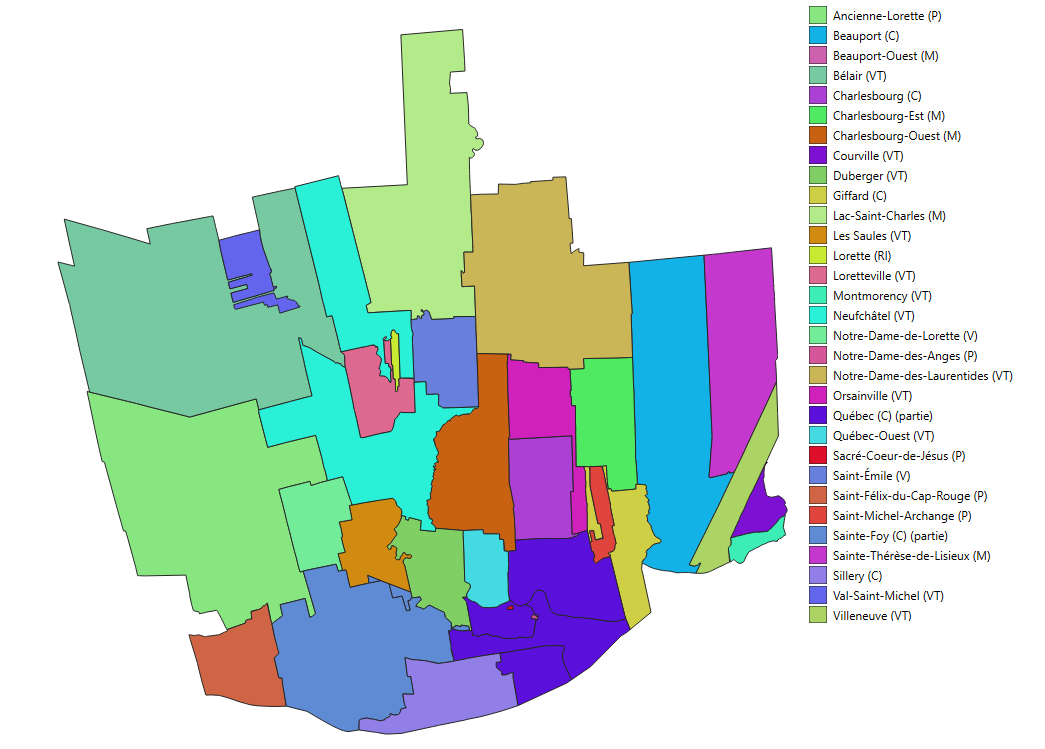
\includegraphics[width=0.9\linewidth]{images/municipalites_1965.png}
    \caption{1965}
    \label{fig:municipalites_1965}
  \end{subfigure}%
  \begin{subfigure}[t]{0.45\textwidth}
    \centering
    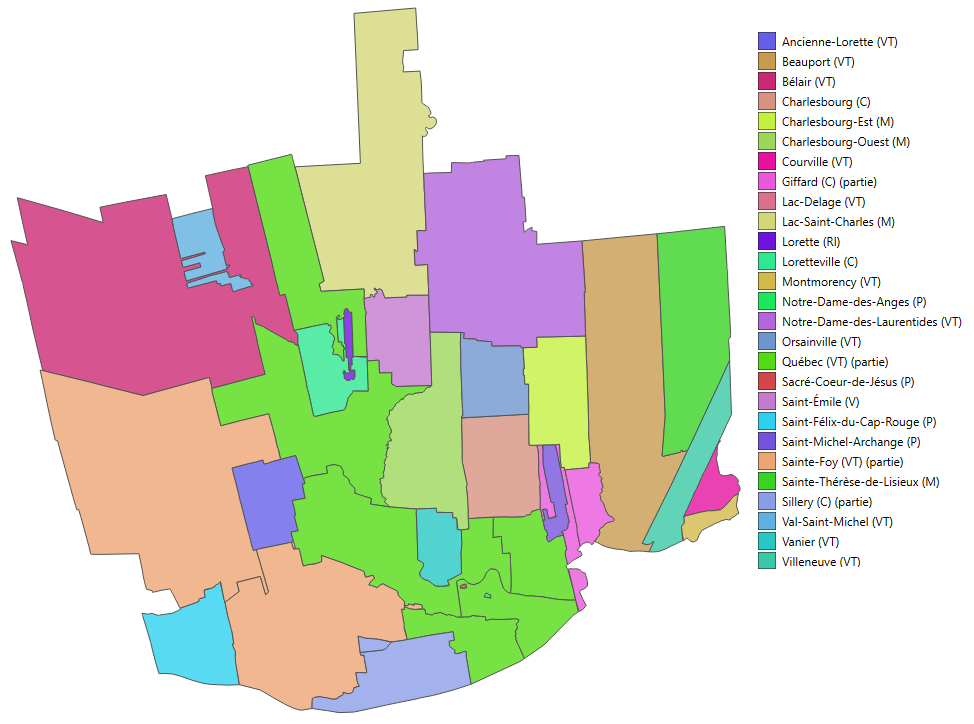
\includegraphics[width=0.9\linewidth]{images/municipalites_1972.png}
    \caption{1972}
    \label{fig:municipalites_1972}
  \end{subfigure}\\
  \begin{subfigure}[t]{0.45\textwidth}
    \centering
    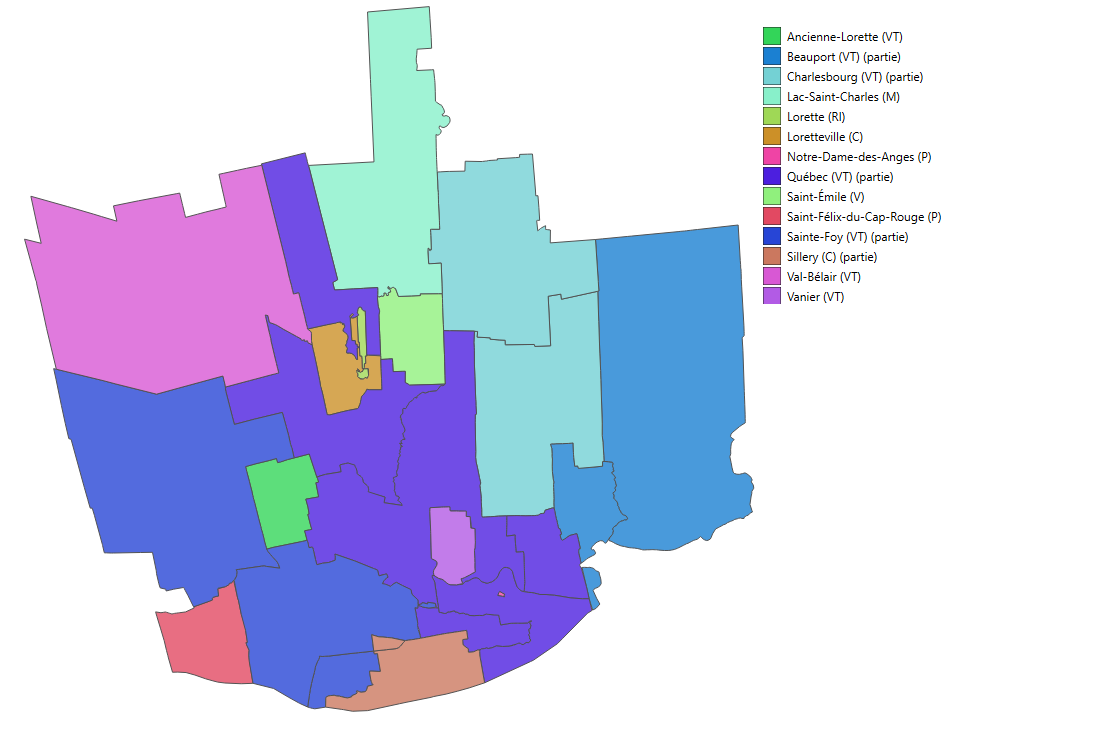
\includegraphics[width=0.9\linewidth]{images/municipalites_1980.png}
    \caption{1980}
    \label{fig:municipalites_1980}
  \end{subfigure}%
  \begin{subfigure}[t]{0.45\textwidth}
    \centering
    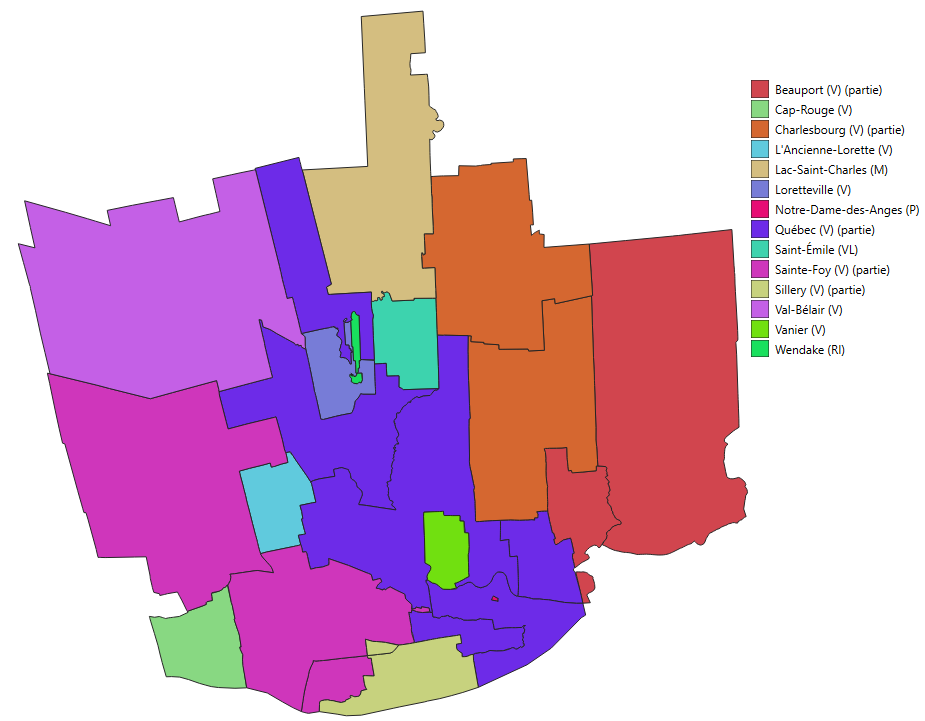
\includegraphics[width=0.9\linewidth]{images/municipalites_1988.png}
    \caption{1988}
    \label{fig:municipalites_1988}
  \end{subfigure}\\
  \begin{subfigure}[t]{0.45\textwidth}
    \centering
    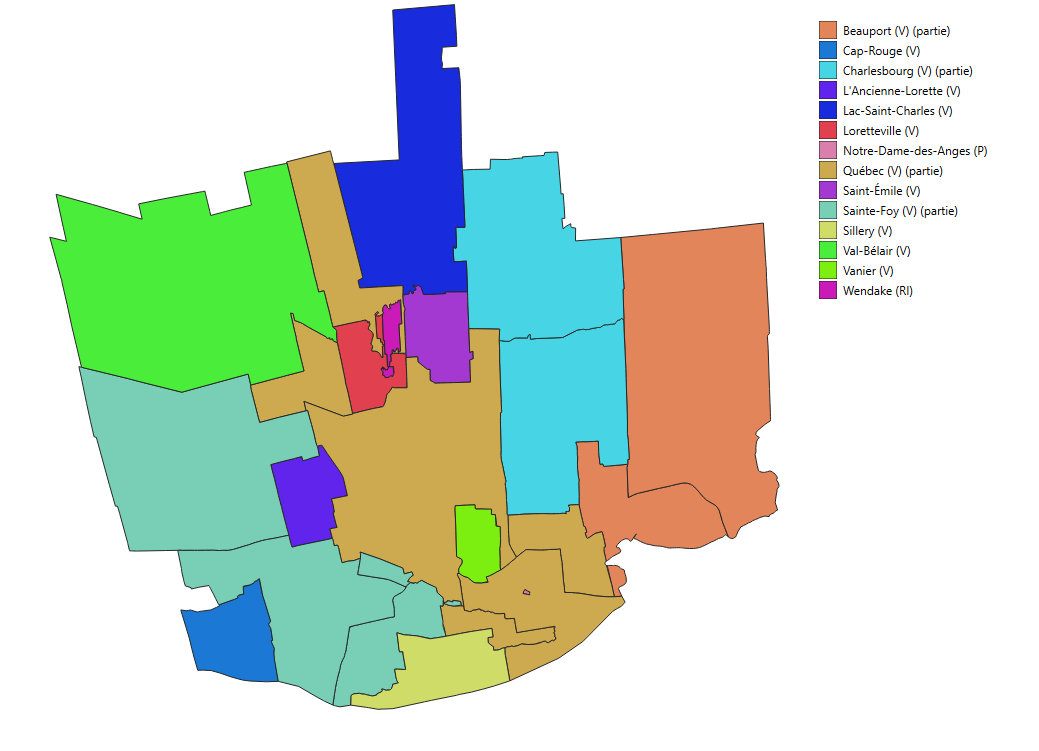
\includegraphics[width=0.9\linewidth]{images/municipalites_2001.png}
    \caption{2001}
    \label{fig:municipalites_2001}
  \end{subfigure}%
  \begin{subfigure}[t]{0.45\textwidth}
    \centering
    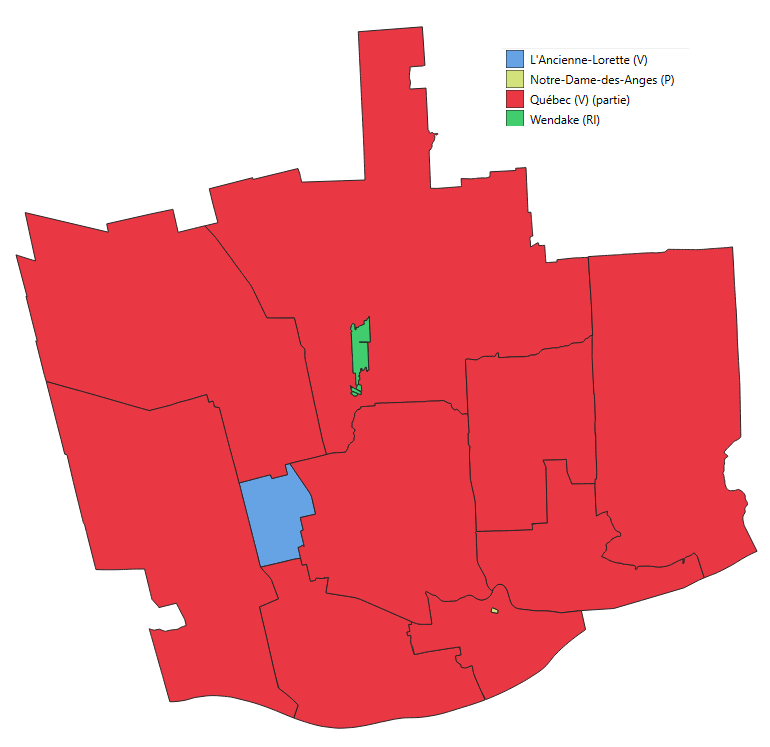
\includegraphics[width=0.8 \linewidth]{images/municipalites_2011.png}
    \caption{2011}
    \label{fig:municipalites_2011}
  \end{subfigure}%
  \caption{Séparation géopolitique du territoire de l'actuelle Ville de Québec \parencite{ElectionsQuebec:AtlasHistorique:2021}}\label{fig:municipalites_carto_historique}
\end{figure}

%Cela étant dit, l'historique de fusion de municipalités et la difficulté de trouver des codes d'urbanisme avant 1995 rend l'utilisation de ces données relativement difficile. La figure \ref{fig:historique_fusions} montre les fusions successives ayant mené à l'actuelle ville de Québec:
  %\begin{figure}[!h]
  %  \centering
  %  \captionsetup{justification=centering,margin=2cm}
  %  \includegraphics[width = 0.5\textwidth]{images/historique_fusions_VDQ.png}
  %  \captionsetup{justification=centering,margin=2cm}
  %  \caption{Diagramme montrant les fusions géopolitiques de la ville de Québec. \hl{Vérifier droits d'auteurs} Source: }
  %  \label{fig:historique_fusions}
  %\end{figure}
  %\FloatBarrier

%D'autre part, à travers les années '90, la ville de Québec va créer des requis de statinnement différents par quartiers. Post-fusion, les différentes villes garderont leurs codes d'urbanisme jusqu'en 2009 où la ville créera un code applicable à l'ensemble du territoire avec 4 sous zone: Général, Axe Structurant B, Axe Structurant A et Urbain Dense \parencite{VilledeQuebec:ReglementHarmonisation:2009}. La définition spatiale des unités de voisinage est donnée dans \textcite{VilledeQuebec:ZonageMunicipal:2024} et l'assignation de la zone est donnée dans \textcite{VilledeQuebec:GrilleSpecifications:2024}. La carte à la figure \ref{fig:types_unites_voisinage} montre les unités de voisinage pour la ville de Québec catégorisé selon la définition ci-haut:
\begin{figure}[ht]
  \centering
  \begin{subfigure}[t]{0.5\textwidth}
    \centering
    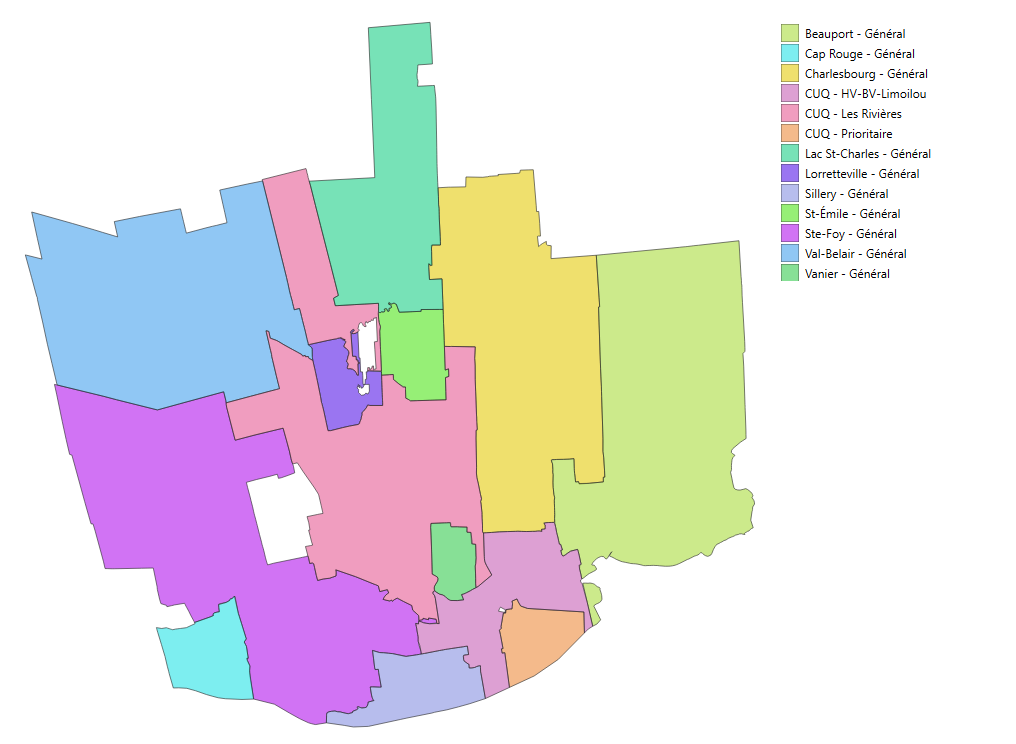
\includegraphics[width=0.9\linewidth]{images/geographie_code_urbanisme_1995-1997.png}
    \caption{1995-1997}
  \end{subfigure}~
  \begin{subfigure}[t]{0.5\textwidth}
    \centering
    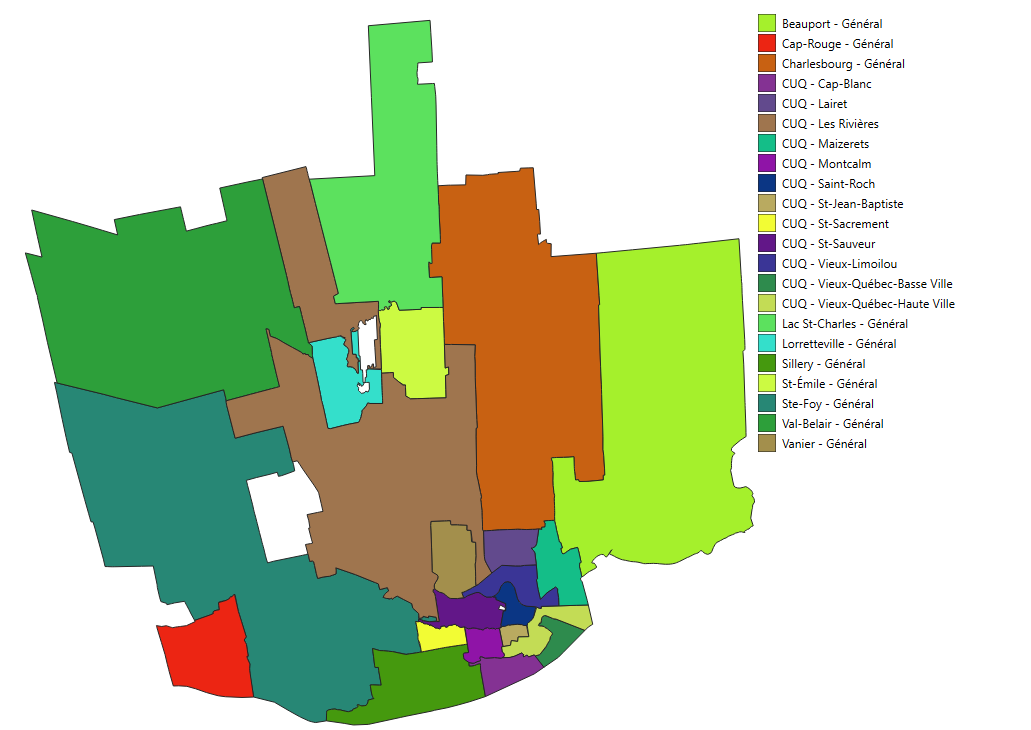
\includegraphics[width=0.9\linewidth]{images/geographie_code_urbanisme_1997-2009.png}
    \caption{1995-1997}
  \end{subfigure}\\
  \begin{subfigure}[t]{0.6\textwidth}
  \centering
  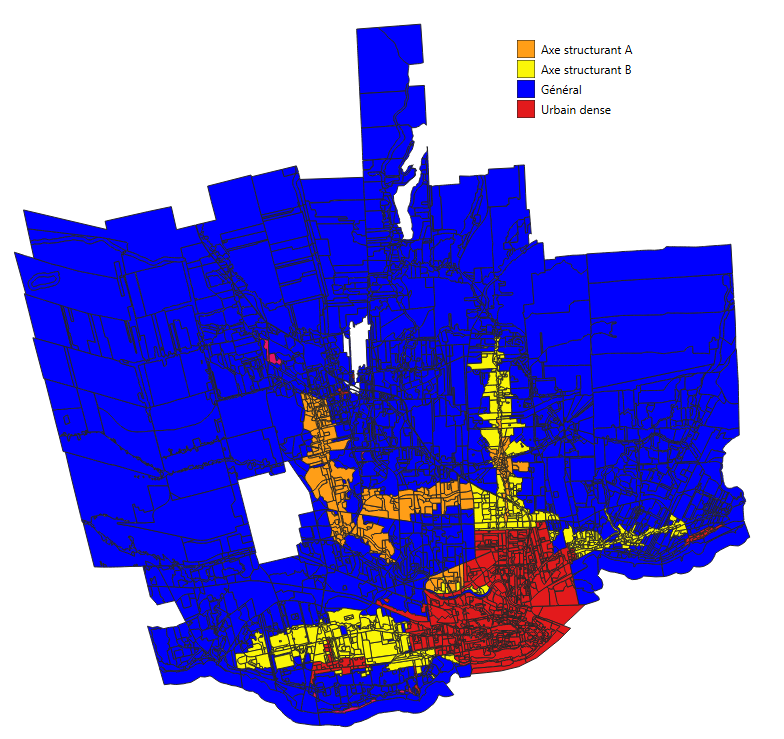
\includegraphics[width=0.8\linewidth]{images/geographie_code_urbanisme_2009_present.png}
  \caption{2010-présent}
  \end{subfigure}
  \caption{Secteur ayant des minimum de stationnement différents}
  \label{fig:types_unites_voisinage}
\end{figure}
\FloatBarrier
\section{Politiques de stationnement de la ville de Québec} \label{sec:politiques_stationnement}

La ville de Québec est en processus d'abroger ces requis pour l'habitation pour les zones en milieu dense ou le long des axes de transport en commun \parencite{VilledeQuebec:AdoptionReglement:2024}.\par
  En plus de l'hétérogénéité spatiale qui est décrite à la section \ref{sec:geopolitique_quebec}, on constate aussi une hétérogénéité au niveau des catégories utilisées pour les requis de stationnement. Ceci est d'autant plus ardu que les catégories utilisées dans les minimums de stationnement n'ont pas nécessairement d'équivalent direct dans le \ac{CUBF} utilisé dans le rôle foncier du Québec \parencite[Annexe 2C.1]{GouvernementduQuebec:ManuelEvaluation:2024}. Le tableau \ref{tab:req_stat_presents} et la figure \ref{fig:n_utilisation_CUBF_minimums} résument la présence d'un requis de stationnement explicité ou inféré pour un code \ac{CUBF} donné \parencite{VilledeQuebec:AdoptionReglement:2024,VilledeQuebec:ReglementZonage:1995}. Les codes d'urbanisme des municipalités pré-fusion sont issus d'un résumé fourni par la ville. Cette synthèse est nécessairement arbitraire: les catégories dans le code d'urbanisme ne sont pas constantes entre les codes avec différents niveaux de superposition ou catégorisation par municipalité, rendant une synthèse difficile. La synthèse est recalée sur les codes \ac{CUBF} pour la simple raison que cette donnée sera exploitée pour choisir la réglementation à appliquer pour inférer une capacité de stationnement requise. Les données sont issues d'une synthèse de la ville. Une demande a été complétée auprès du service de greffe pour obtenir les textes de loi.
  %\tiny
  \newcommand{\YCHECK}{\Checkmark}
  \newcommand{\NCHECK}{\cellcolor{red} \XSolid}
  \newcommand{\OCHECK}[1]{\cellcolor{orange} / #1}
  \newcolumntype{P}[1]{>{\centering\arraybackslash}p{#1}}
  \newcolumntype{M}[1]{>{\centering\arraybackslash}m{#1}}
  
  \setlength{\LTcapwidth}{\textwidth}
  \begin{landscape}
    \begin{center}
      \begin{longtable}{P{1.0cm} | p{7.5cm} | c || *{12}{P{5mm}}||p{6mm}} 
        \multirow{2}{*}{\STAB{\rotatebox[origin=c]{90}{Categ}}} & Juridiction & \STAB{\rotatebox[origin=c]{90}{Code \ac {CUBF}}} & \rotatebox[origin=c]{90}{  VDQ (2009-présent)} & \rotatebox[origin=c]{90}{VDQ (1995-2009)} & \rotatebox[origin=c]{90}{Beauport} & \rotatebox[origin=c]{90}{Cap-Rouge} & \rotatebox[origin=c]{90}{Charlesbourg} & \rotatebox[origin=c]{90}{Lac St-Charles} & \rotatebox[origin=c]{90}{Loretteville} & \rotatebox[origin=c]{90}{Sillery} & \rotatebox[origin=c]{90}{Ste-Foy} & \rotatebox[origin=c]{90}{St-Émile} & \rotatebox[origin=c]{90}{Val-Belair} & \rotatebox[origin=c]{90}{Vanier} & \rotatebox[origin=c]{90}{Nombre de requis} \\
        %& No. Règl. & MEFQ & R.V.Q. 1400 & V.Q.Z. 3 & 87-806 & 1151-95 & 96-2921 & 88-257 & 1386 & 950 & 3501 & 310-89 & VB-344-88 & 93-05-1245\\
        \hline  
        \endhead
        \hline
        \multicolumn{15}{c}{\Checkmark = Requis présent, \colorbox{red}{\XSolid} = Requis absent, \colorbox{orange}{/} = Requis implicite à une définition plus générale}\\\hline
        \endfoot
        \hline
        \multicolumn{15}{c}{\Checkmark = Requis présent, \colorbox{red}{\XSolid} = Requis absent, \colorbox{orange}{/} = Requis implicite à une définition plus générale}\\\hline
        \caption{Présence de règlementation de stationnement selon le code \ac{CUBF}}\label{tab:req_stat_presents}
        \endlastfoot
        \multirow{6}{*}{\STAB{\rotatebox[origin=c]{90}{Résidentiel}}} & Logement & 10XX & \YCHECK & \YCHECK &\YCHECK & \YCHECK &\YCHECK &\YCHECK& \YCHECK & \YCHECK & \YCHECK &\YCHECK & \YCHECK & \YCHECK&12\\
        & Logement subventionné & 10XX & \YCHECK & \YCHECK & \NCHECK & \NCHECK & \NCHECK& \NCHECK &\NCHECK &\NCHECK &\NCHECK &\NCHECK &\NCHECK & \NCHECK&2 \\
        & Habitation Collectives & 15XX & \YCHECK & \NCHECK & \YCHECK & \YCHECK & \YCHECK & \YCHECK & \YCHECK & \NCHECK & \NCHECK & \YCHECK & \YCHECK & \NCHECK&8 \\
        & Maison de chambres &  151X & \YCHECK & \YCHECK & \OCHECK{} & \OCHECK{} & \OCHECK{} & \OCHECK{} & \YCHECK & \NCHECK & \YCHECK &\OCHECK{} & \YCHECK & \YCHECK&6\\
        & Maison de retraite non autonomes & 1541 & \OCHECK{} & \YCHECK & \YCHECK & \YCHECK & \OCHECK{} & \OCHECK{} & \YCHECK & \YCHECK & \YCHECK & \OCHECK{} & \OCHECK{} & \NCHECK &6\\
        & Maison de retraite autonomes & 1543 & \OCHECK{} & \YCHECK & \YCHECK & \YCHECK & \OCHECK{} & \OCHECK{} & \YCHECK & \YCHECK & \YCHECK & \OCHECK{} & \OCHECK{} & \NCHECK&6 \\ 
        \hline
        \multirow{7}{*}{\STAB{\rotatebox[origin=c]{90}{Industriel / Infra.}}}& Industriel Général & \makecell[l]{2XXX\\3XXX} & \YCHECK & \YCHECK & \YCHECK & \YCHECK & \YCHECK & \YCHECK & \YCHECK & \YCHECK & \YCHECK & \YCHECK & \YCHECK & \YCHECK&12 \\
        & Industrie Haute Technologie & \makecell[l]{355X\\356X\\357X} & \YCHECK & \OCHECK{} & \OCHECK{}  & \OCHECK{}  & \OCHECK{}   & \OCHECK{}   & \OCHECK{}   & \OCHECK{}   &  \YCHECK & \OCHECK{}   & \OCHECK{}& \OCHECK{}&2 \\
        & Industrie mise en valeur et récupération &487X & \YCHECK & \OCHECK{} & \OCHECK{} & \OCHECK{} & \OCHECK{} & \OCHECK{} & \OCHECK{} & \OCHECK{} & \YCHECK & \OCHECK{} & \OCHECK{} & \OCHECK{}&2 \\ 
        & Entreposage & 637X & \YCHECK&\YCHECK&\OCHECK{}&\OCHECK{}&\OCHECK{}&\OCHECK{}&\YCHECK&\YCHECK&\OCHECK{}&\YCHECK&\YCHECK&\YCHECK &7\\
        & Service de construction & 66XX & \OCHECK{}  & \OCHECK{} &\OCHECK{} &\OCHECK{} &\OCHECK{} &\OCHECK{} & \YCHECK &\OCHECK{} &\OCHECK{} & \OCHECK{} & \OCHECK{} & \YCHECK&2\\
        \hline
        \multirow{4}{*}{\STAB{\rotatebox[origin=c]{90}{Commerces}}} & Centre et Immeuble Commercial & 50XX & \YCHECK & \YCHECK & \YCHECK & \YCHECK &\YCHECK&\YCHECK& \YCHECK&\YCHECK&\YCHECK&\YCHECK&\YCHECK&\YCHECK&12\\
        & Vente en gros & 51XX &\OCHECK{}&\YCHECK&\OCHECK{}&\OCHECK{}&\OCHECK{}&\OCHECK{}&\YCHECK&\OCHECK{}&\OCHECK{}&\OCHECK{}&\YCHECK&\OCHECK{}&3\\
        & Vente au détail construction et quincaillerie & 52XX&\OCHECK{}&\OCHECK{}&\OCHECK{}&\YCHECK&\OCHECK{}&\OCHECK{}&\YCHECK&\YCHECK&\YCHECK&\OCHECK{}&\YCHECK&\OCHECK{}&5 \\
        & Vente au détail marchandises & 53XX&\OCHECK{}&\OCHECK{}&\OCHECK{}&\OCHECK{}&\OCHECK{}&\OCHECK{}&\OCHECK{}&\OCHECK{}&\OCHECK{}&\OCHECK{}&\OCHECK{}&\OCHECK{}&0\\
        \multirow{6}{*}{\STAB{\rotatebox[origin=c]{90}{Commerces}}} & Vente au détail de l'alimentation & 54XX &\YCHECK&\YCHECK&\OCHECK{}&\OCHECK{}&\YCHECK&\YCHECK&\YCHECK&\YCHECK&\YCHECK&\YCHECK&\YCHECK&\YCHECK &10\\
        & Vente au détail de véhicules et produits connexes & 55XX &\YCHECK&\OCHECK{}&\OCHECK{}&\OCHECK{}&\OCHECK{}&\YCHECK&\YCHECK&\YCHECK&\YCHECK&\YCHECK&\YCHECK&\YCHECK&8\\
        & Station Essence & 553X&\YCHECK&\YCHECK&\YCHECK&\OCHECK{}&\OCHECK{}&\OCHECK{}&\YCHECK&\OCHECK{}&\YCHECK&\YCHECK&\YCHECK&\YCHECK&7 \\
        & Vente au détail de vêtements & 56XX&\OCHECK{}&\OCHECK{}&\OCHECK{}&\OCHECK{}&\OCHECK{}&\OCHECK{}&\YCHECK&\OCHECK{}&\YCHECK&\OCHECK{}&\OCHECK{}&\OCHECK{}&2\\
        & Vente au détail de mobilier & 57XX&\YCHECK&\YCHECK&\OCHECK{}&\OCHECK{}&\OCHECK{}&\OCHECK{}&\YCHECK&\OCHECK{}&\OCHECK{}&\OCHECK{}&\OCHECK{}&\OCHECK{}&3 \\
        & Vente au détail Autre & 59XX&\OCHECK{}&\OCHECK{}&\OCHECK{}&\OCHECK{}&\OCHECK{}&\OCHECK{}&\OCHECK{}&\OCHECK{}&\OCHECK{}&\OCHECK{}&\OCHECK{}&\OCHECK{}&0\\
        \hline
        \multirow{7}{*}{\STAB{\rotatebox[origin=c]{90}{Restaurants et bars}}} & Restaurant & 581X & \YCHECK&\NCHECK&\YCHECK&\NCHECK&\YCHECK&\YCHECK&\YCHECK&\YCHECK&\YCHECK &\YCHECK&\YCHECK&\YCHECK&7 \\
        & Restaurant plein service & \makecell{5811 \\ 5812 \\ 5815}& \OCHECK{}&\YCHECK&\OCHECK{}&\YCHECK&\OCHECK{}&\OCHECK{}&\OCHECK{}&\OCHECK{}&\OCHECK{}&\OCHECK{}&\OCHECK{}&\OCHECK{}&2\\
        & Restaurant service restreint/libre service& \makecell{5811 \\ 5812 }& \OCHECK{}&\YCHECK&\OCHECK{}&\YCHECK&\OCHECK{}&\OCHECK{}&\OCHECK{}&\OCHECK{}&\OCHECK{}&\OCHECK{}&\OCHECK{}&\OCHECK{}&2\\
        & Débit d'alcool & 582X&\YCHECK&\YCHECK&\YCHECK&\YCHECK&\YCHECK&\YCHECK&\YCHECK&\YCHECK&\YCHECK&\YCHECK&\YCHECK&\YCHECK&11\\
        \hline
        \multirow{3}{*}{\STAB{\rotatebox[origin=c]{90}{Tourisme}}} & Établissement d'hébergement & 583X&\YCHECK&\NCHECK&\NCHECK&\YCHECK&\YCHECK&\YCHECK&\YCHECK&\YCHECK&\YCHECK&\YCHECK&\YCHECK&\YCHECK&10\\
        & Hôtel & 5831&\OCHECK{}&\YCHECK&\YCHECK&\OCHECK{}&\OCHECK{}&\OCHECK{}&\OCHECK{}&\OCHECK{}&\OCHECK{}&\OCHECK{}&\OCHECK{}&\OCHECK{}&2\\
        & Môtel & 5832&\OCHECK{}&\YCHECK&\YCHECK&\OCHECK{}&\OCHECK{}&\OCHECK{}&\OCHECK{}&\OCHECK{}&\OCHECK{}&\OCHECK{}&\OCHECK{}&\OCHECK{}&2\\
        \hline
        & Services & 6XXX & \YCHECK & \YCHECK & \YCHECK &\YCHECK & \YCHECK & \YCHECK & \YCHECK & \YCHECK &\YCHECK &\NCHECK &\YCHECK&\NCHECK&10\\
        & Immeubles à bureaux & 60XX&\YCHECK&\YCHECK&\OCHECK{}&\YCHECK&\YCHECK&\YCHECK&\YCHECK&\YCHECK&\YCHECK&\NCHECK&\YCHECK&\NCHECK&9\\
        \multirow{19}{*}{\STAB{\rotatebox[origin=c]{90}{Services}}}& Finance, Assurance et Service immobilier & 61XX&\OCHECK{}&\YCHECK&\OCHECK{}&\OCHECK{}&\OCHECK{}&\OCHECK{}&\YCHECK&\OCHECK{}&\OCHECK{}&\YCHECK&\OCHECK{}&\YCHECK&4\\
        & Banque & 611X&\OCHECK{}&\YCHECK&\OCHECK{}&\YCHECK&\OCHECK{}&\YCHECK&\YCHECK&\YCHECK&\YCHECK&\OCHECK{}&\YCHECK&\OCHECK{}&7\\
        & Service personnels & 62XX & \OCHECK{} &\OCHECK{}&\OCHECK{}&\OCHECK{}&\YCHECK&\OCHECK{}& \OCHECK{}&\OCHECK{}&\YCHECK&\OCHECK{} &\OCHECK{}&\OCHECK{}&2\\
        & Salon de beauté / coiffure& 623X& \OCHECK{}&\YCHECK&\OCHECK{}&\OCHECK{}&\OCHECK{}&\OCHECK{}&\YCHECK&\OCHECK{}&\OCHECK{}&\OCHECK{}&\OCHECK{}&\YCHECK &3\\
        & Salon funéraire& 624X&\YCHECK&\YCHECK&\YCHECK&\YCHECK&\YCHECK&\YCHECK&\YCHECK&\YCHECK&\YCHECK&\YCHECK&\YCHECK&\YCHECK&12\\
        & Services d'affaires & 63XX &\OCHECK{}&\OCHECK{}&\YCHECK&\OCHECK{}&\OCHECK{}&\OCHECK{}&\YCHECK&\OCHECK{}&\OCHECK{}&\YCHECK&\OCHECK{}&\YCHECK&4\\
        & Services de réparation & 64XX&\OCHECK{}&\OCHECK{}&\OCHECK{}&\OCHECK{}&\OCHECK{}&\OCHECK{}&\OCHECK{}&\OCHECK{}&\OCHECK{}&\OCHECK{}&\OCHECK{}&\OCHECK{}&0\\
        & Service de réparation d'automobiles&641X&\YCHECK&\YCHECK&\YCHECK&\YCHECK&\OCHECK{}&\OCHECK{}&\YCHECK&\OCHECK{}&\YCHECK&\YCHECK&\YCHECK&\YCHECK&9\\
        & Service de réparation de mobiliers, d'équipements et de machines & 642X&\OCHECK{}&\OCHECK{}&\OCHECK{}&\OCHECK{}&\OCHECK{}&\OCHECK{}&\YCHECK&\OCHECK{}&\OCHECK{}&\OCHECK{}&\OCHECK{}&\OCHECK{}&1\\ 
        & Service de réparation de véhicules légers& 643X&\YCHECK&\YCHECK&\YCHECK&\YCHECK&\OCHECK{}&\OCHECK{}&\YCHECK&\OCHECK{}&\YCHECK&\YCHECK&\YCHECK&\YCHECK&9\\
        & Service de réparation et d'entretien de véhicules lourds& 644X&\YCHECK&\YCHECK&\YCHECK&\YCHECK&\OCHECK{}&\OCHECK{}&\YCHECK&\OCHECK{}&\YCHECK&\YCHECK&\YCHECK&\YCHECK&9\\
        & Service professionnel & 65XX&\YCHECK&\OCHECK{}&\YCHECK&\YCHECK&\OCHECK{}&\OCHECK{}&\OCHECK{}&\OCHECK{}&\OCHECK{}&\OCHECK{}&\OCHECK{}&\OCHECK{}&0\\
        & Service médical et de santé & 651X&\YCHECK&\YCHECK&\OCHECK{}&\OCHECK{}&\YCHECK&\YCHECK&\YCHECK&\YCHECK &\YCHECK & \OCHECK{} &\YCHECK & \OCHECK{}&9\\
        & Service d'hôpital & 6513 &\YCHECK &\YCHECK &\YCHECK &\YCHECK&\YCHECK&\YCHECK&\YCHECK&\YCHECK&\YCHECK&\YCHECK&\YCHECK&\YCHECK&12\\
        & Sanatorium, maison de convalescence et de repos & 6516 &\YCHECK &\YCHECK &\YCHECK&\OCHECK{}&\YCHECK &\YCHECK&\YCHECK&\YCHECK&\YCHECK&\YCHECK&\YCHECK&\YCHECK&11\\
        \multirow{12}{*}{\STAB{\rotatebox[origin=c]{90}{Services}}}& Service gouvernemental&67XX&\OCHECK{} & \OCHECK{} &\OCHECK{}&\OCHECK{}&\OCHECK{} &\OCHECK{} & \YCHECK&\OCHECK{}&\YCHECK&\YCHECK&\YCHECK&\YCHECK &5 \\
        & Pompiers/Police &672X&\YCHECK & \YCHECK &\OCHECK{}&\OCHECK{} &\OCHECK{} & \OCHECK{}&\OCHECK{}&\YCHECK&\OCHECK{}&\YCHECK&\OCHECK{}&\OCHECK{}&4\\
        & Service éducationnel&68XX&\YCHECK&\YCHECK&\NCHECK&\YCHECK&\NCHECK&\YCHECK&\YCHECK&\YCHECK&\NCHECK&\YCHECK{}&\YCHECK&\YCHECK &9 \\
        & Service de garderie&6541&\YCHECK&\OCHECK{}&\OCHECK{}&\OCHECK{}& \YCHECK&\OCHECK{}& \YCHECK &\OCHECK{}&\YCHECK&\OCHECK{}&\YCHECK&\OCHECK{}&5 \\
        & École Maternelle&6811&\OCHECK{}&\OCHECK{}&\OCHECK{}&\OCHECK{}&\OCHECK{}&\OCHECK{}&\YCHECK&\OCHECK{}&\YCHECK&\OCHECK{}&\YCHECK{}&\YCHECK{}&4 \\
        & École Primaire&6812&\YCHECK&\YCHECK&\YCHECK&\YCHECK&\YCHECK&\YCHECK&\YCHECK&\YCHECK&\YCHECK&\OCHECK{}&\YCHECK&\YCHECK&11 \\
        & École Secondaire / Polyvalente&\makecell{6813\\6822}&\YCHECK&\YCHECK&\YCHECK&\OCHECK{}&\YCHECK& \YCHECK&\YCHECK&\YCHECK&\YCHECK&\OCHECK{}&\YCHECK&\YCHECK&10 \\
        & CÉGEP &6823&\YCHECK&\YCHECK&\YCHECK&\OCHECK{}&\OCHECK{}&\YCHECK&\YCHECK&\OCHECK{}&\YCHECK&\OCHECK{}&\OCHECK{}&\OCHECK{}&6\\
        & Université&6821&\YCHECK&\YCHECK&\YCHECK&\OCHECK{}&\YCHECK&\YCHECK&\YCHECK&\OCHECK{}&\YCHECK&\OCHECK{}&\OCHECK{}&\OCHECK{}&7\\ 
        & Services religieux &691X&\YCHECK&\OCHECK{}&\YCHECK&\YCHECK&\OCHECK{}&\YCHECK&\YCHECK&\YCHECK&\YCHECK&\OCHECK{}&\YCHECK&\YCHECK&9\\
        \hline
        \multirow{8}{*}{\STAB{\rotatebox[origin=c]{90}{Culture et Récréation}}} & Culture, Récréation et Loisirs&7XXX &\NCHECK&\YCHECK&\YCHECK&\NCHECK&\YCHECK&\YCHECK&\NCHECK&\YCHECK&\NCHECK&\YCHECK&\YCHECK&\YCHECK&8\\
        & Activité Culturelle(Musée, Biblio) &711X&\YCHECK&\YCHECK&\YCHECK&\YCHECK&\YCHECK&\YCHECK&\YCHECK&\YCHECK&\YCHECK &\OCHECK{} &\OCHECK{} &\OCHECK{}&9\\
        & Assemblée de loisirs(Théâtre, Cinéma) &721X&\YCHECK&\YCHECK&\YCHECK& \YCHECK& \YCHECK&\YCHECK&\YCHECK&\YCHECK&\YCHECK&\OCHECK{}&\YCHECK&\OCHECK{}&10 \\
        & Installation sportive (Stade, Hippodrome)&722X&\YCHECK&\OCHECK{}&\OCHECK{}&\NCHECK&\OCHECK{}&\OCHECK{}&\YCHECK&\OCHECK{}&\YCHECK&\OCHECK{}&\OCHECK{}&\OCHECK{}&3\\
        & Centre de congrès&723X& \OCHECK{} & \YCHECK & \OCHECK{} & \NCHECK & \OCHECK{} & \OCHECK{}& \YCHECK& \OCHECK{} & \OCHECK{} & \OCHECK{} & \OCHECK{} & \OCHECK{}&2 \\
        & Activités récréatives&74XX&\YCHECK&\OCHECK{}&\YCHECK&\NCHECK&\OCHECK{}&\OCHECK{}&\YCHECK&\OCHECK{}&\YCHECK&\OCHECK{}&\OCHECK{}&\OCHECK{} &4\\
        & Terrains de golf&\makecell{7411\\7412}& \YCHECK& \OCHECK{}&\OCHECK{}&\NCHECK&\OCHECK{}&\OCHECK{}&\YCHECK&\OCHECK{}&\YCHECK&\YCHECK&\OCHECK{}&\OCHECK{}&4\\
        & Arena& 7451& \YCHECK&\YCHECK&\OCHECK{}&\NCHECK&\OCHECK{}&\OCHECK{}&\YCHECK{}&\YCHECK&\OCHECK{}&\YCHECK&\YCHECK&\OCHECK{}&6\\
        & Parcs/Camps &\makecell{75XX\\76XX}&\YCHECK &\NCHECK&\NCHECK&\NCHECK&\NCHECK&\NCHECK&\NCHECK&\NCHECK&\YCHECK&\YCHECK&\NCHECK&\YCHECK&5 \\
        \hline
        N/A & Extraction de ressources / Agriculture & 8XXX&\YCHECK&\NCHECK&\NCHECK&\NCHECK&\NCHECK&\NCHECK&\YCHECK&\NCHECK&\YCHECK&\NCHECK&\NCHECK&\NCHECK&3\\
      \end{longtable}
    \end{center}  
    \begin{figure}[h]
      \centering
      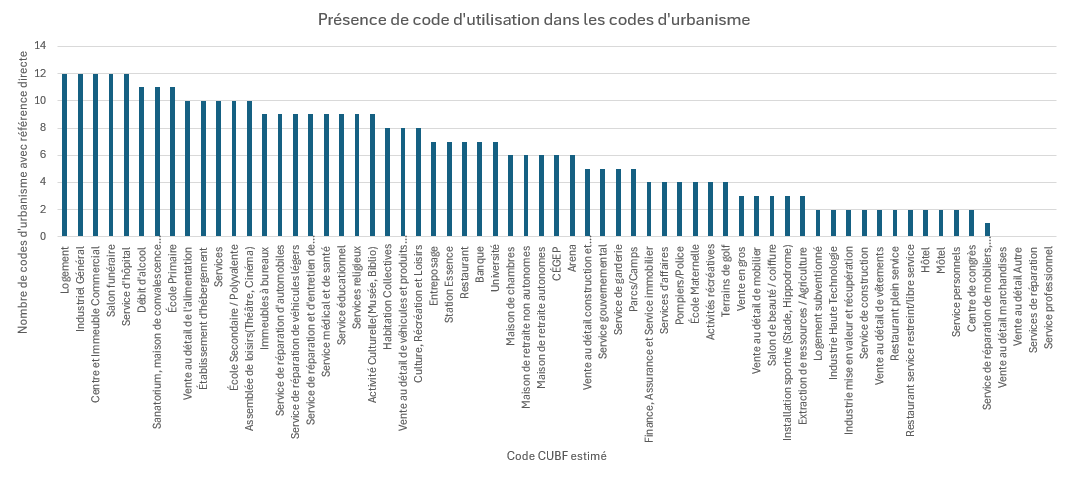
\includegraphics[width=22cm]{images/presence_requis_par_CUBF}
      \caption{Nombre de codes d'urbanisme utilisant les codes d'utilisation listés}\label{fig:n_utilisation_CUBF_minimums}
    \end{figure}
  \end{landscape}
  %\normalsize
  \FloatBarrier
  
  Les objets sur lesquels sont basés les codes d'urbanisme sont aussi hétérogènes. Bien que la plupart des requis soient basé sur une surface de plancher, certains sont exprimés en fonction d'autres objets considérés pertinents. D'autre part, la même utilisation du sol n'est pas nécessairement légiférée en utilisant le même objet entre deux juridictions différentes. Le tableau \ref{tab:objet_pour_inference_capacite} synthétise les objets considérés et les usages pour lesquels ils sont utilisés.

  \begin{table}[h]
    \centering
    \begin{tabular}{p{4cm} p{8cm}}
      \hline
      Objets considéré & Usages pertinents \\
      \hline
      Superficie de plancher & Majoritaire\\
      Superficie par usage (bureau, plateau TV) & Station télé \\
      Superficie de terrain & parc, zoo \\
      Logement & Logement \\
      Chambres & Maison de chambres, hébergement touristique, établissement de santé\\
      Lit & Établissement de santé, auberges de jeunesse, établissement carcéral \\
      Baie de service & Commerces liés à l'automobile\\
      Siège & Lieux de rassemblement, cinéma, théâtres, stades \\
      Salle & Cabinet médical, établissement scolaire, salon funéraire\\
      Personne & Débit d'alcool\\
      Employé & Services et vente au détail\\
      Médecin & Établissement de santé\\
      Étudiant & Établissement scolaire\\
      Plateau sportif & Golf, tennis, quilles, billards\\
      Poste de travail & Services personnels (salon de beauté)\\
      \hline
    \end{tabular}
    \caption{Récapitulatif des objets considérés pour fixer les capacité de stationnement}\label{tab:objet_pour_inference_capacite}
  \end{table}
  

  \FloatBarrier

\section{Données de départ}\label{sec:meth_donnees_dispo}
  \subsection{\ac{SIG}}
    \subsubsection{Synthèse des données disponibles}
      Le tableau \ref{tab:donnees_disponibles_Québec} résume les données disponibles pour la ville de Québec et leur source.
      \begin{landscape}
        \LTcapwidth=\textwidth
      \begin{longtable}[h!]{p{.2 \linewidth} p{.1 \linewidth} p{.3 \linewidth} p{.15\linewidth} p{.125\linewidth} }
        
        
        \hline
        Géobase & Type & Description  & Source & Date téléchargement.\\ 
        \hline
        \hline
        \endhead
        \hline
        \endfoot
        \hline
        \caption{Géobases pour le territoire de la ville de Québec}
        \label{tab:donnees_disponibles_Québec}
        \endlastfoot
        vdq-panneaux stationnement    & Points        & Panneaux de stationnement sur rue          & Ville de Québec / Données Québec  & 5 mai 2024 \\
        \hline
        vq\_quartiers & Polygones & SIG des quartiers de la ville de Québec & Ville de Québec / Données Québec & 5 mai 2024 \\
        \hline
        vdq-bornesfontaines          & Points        & Borne-fontaine sur rue                   & Ville de Québec / Données Québec & 12 mai 2024 \\
        \hline
        vq\_reseau\_routier\_2023 & Polylignes    & Bords de voiries pour circulation automobile  & Ville de Québec / Geo-index  & 12 juin 2023\\ 
        \hline
        vq\_stationnement\_2021  & Polylignes    & Bords des aires de stationnement hors rue & Ville de Québec / Geo-index & 8 mai 2021\\
        \hline
        vdq\_voie\_publique            & Lignes        & Centres de chaussées, trottoirs séparés et pistes cyclables & Ville de Québec / Données Québec & 16 avril 2024 \\
        \hline
        vdq-zonage-grille.xlsx          & Tableau        & Usages autorisés et classification (urbain/structurant/général) & Ville de Québec / Données Québec & 8 juin 2024 \\
        \hline
        vdq-zonagemunicipalzones          & Polygones        & Unités de voisinages selon le zonage municipal & Ville de Québec / Données Québec & 6 mai 2024 \\
        \hline
        vdq\_intersection\_voie \_publique & Points & Intersections avec les dispositifs de contrôle & Ville de Québec / Données Québec & 8 mai 2024 \\
        \hline
        vdq\_quartiers & Polygones &Séparation de la ville en quartiers & Ville de Québec / Données Québec & 8 mai 2024\\
        \hline
        Usages prédominants 2023  & Polygones & Usages prédominants du sol &   Ministère des Affaires municipales et de l'Habitation & 21 mai 2024 \\
        \hline
        Arrêts bus et à vélo 2024 & Points et polylignes & Arrêts de bus, parcours des lignes et bornes vélopartage & Réseau de transport de la capitale & 31 mai 2023 \\
        \hline
        Année de construction des chaussées & Polylignes & Année de construction des rues & Ville de Québec / Géoindex & 28 mai 2024 \\
        \hline
        Rôle foncier & Entrées de tableaux & Données en format xml du rôle foncier & Ministère des Affaires municipales et de l'Habitation & 28 mai 2024 \\
        \hline
        Rôle foncier géobase & FGDB (Points + tables) & Données SIG du rôle foncier & Ministère des Affaires municipales et de l'Habitation & 28 mai 2024 \\
        \hline
        highway & Polylignes & Centres de chaussées & \ac{OSM} & 13 mai 2024\\
        \hline
        parking & points et polygones & Stationnement recensés dans \ac{OSM} & \ac{OSM} & 2 mai 2024 \\
        \hline
          parking entrance & Points & Entrées de stationnement sous-terrains  & \ac{OSM} & 2 mai 2024 \\
          \hline
        
      \end{longtable}

      \begin{table}[h!]
        \centering
        \begin{tabular}{p{0.18\linewidth} | p{0.1\linewidth} | p{0.3\linewidth} | p{0.3\linewidth}} 
        \hline
        Nom du champs & Type Contenu & Description  & Exemple\\ 
        \hline
        ID             & Entier    & Entier identifiant unique pour chaque panneau  & 370758 \\ 
        & & & \\
        TYPE\_CODE      & Texte     & Code d'identification de chaque type de panneau de stationnement & PP1016\\
        & & & \\
        DESCRIPTION     & Texte     & Texte imprimé sur le panneau & Stat. int. 16h-18h LUN À VEN (fl. dou.)\\
        \hline
        \end{tabular}
        \caption{Champs de la géobase de panneaux de stationnement de la ville de Québec \parencite{VilledeQuebec:PanneauxSignalisation:2024}}
        \label{tab:champs_geobase_stationnement_quebec}
      \end{table}
      \end{landscape}
    \subsubsection{Illustration - Cas 1: Coin Gomin / Marguerite-Bourgeoys / Laurier}
    La section suivante va donner un aperçu de quelques intersections typiques pour illustrer les données disponibles. Le but principal est d'illustrer les enjeux.
      Les figures \ref{fig:donnes_panneaux_Laurier} et \ref{fig:donnes_polygone_panneaux_Laurier} donnent un aperçu des données disponibles pour l'intersection nommée ci-dessus. On constate que plusieurs panneaux sur un même poteau ne sont pas représentés géographiquement au même endroit. D'autre part, la présence de panonceaux donne des exceptions aux limitations de temps de stationnement. De plus, la ville a à sa disposition une géobase de bords de rue, mais aucune information n'est disponible pour associer le bord de rue à un tronçon donné. Le même constat est possible pour les panneaux de stationnement dont les seules informations sont un identifiant, la description et un identifiant de panneau. Ils ne sont pas associés à un tronçon ou un côté de rue. L'une des conséquences de la dispersion des panneaux est aussi la difficulté d'assigner les panneaux à un tronçon aux intersections puisque le panneau peut être plus proche d'un bord de rue autre du fait du décalage des panneaux dans l'espace. Dans ce cas-ci, le panneau Stat. int. (fl. ga.) est à 6m de la rue Marguerite Bourgeoys et 9m de la rue Gomin.
      \begin{figure}[ht]
        \centering
        \begin{subfigure}{\linewidth}
          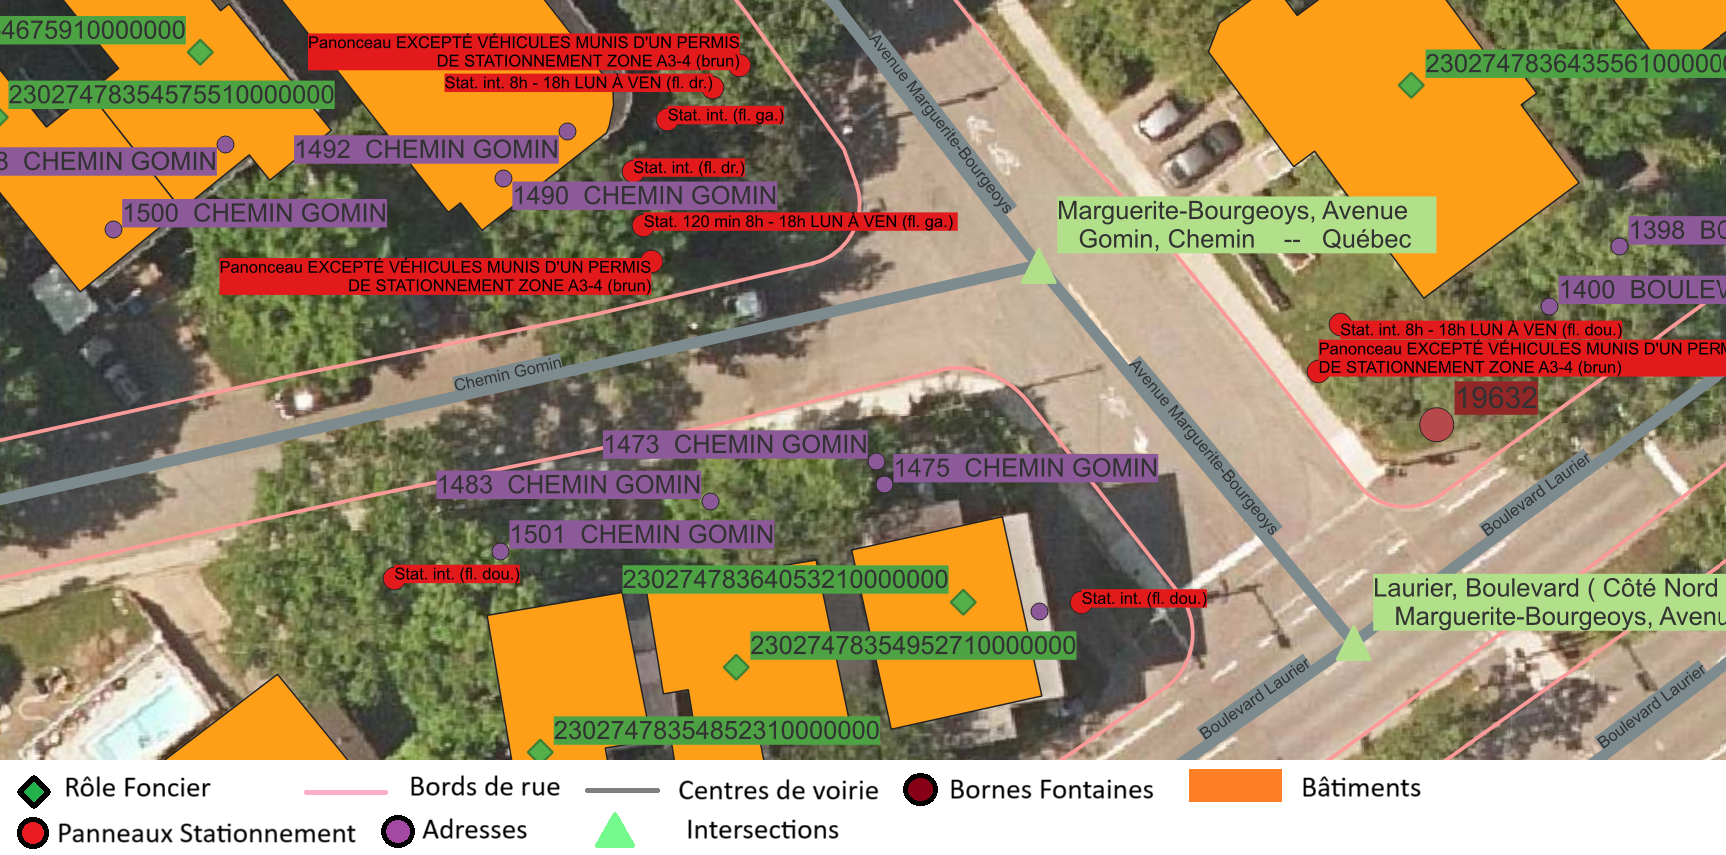
\includegraphics[width=1.0\textwidth]{images/donnees_disponible_Laurier_legende_v2.png}
        \caption{Données linéaires disponibles}
        \label{fig:donnes_panneaux_Laurier}
        \end{subfigure} \\
        \begin{subfigure}{\linewidth}
          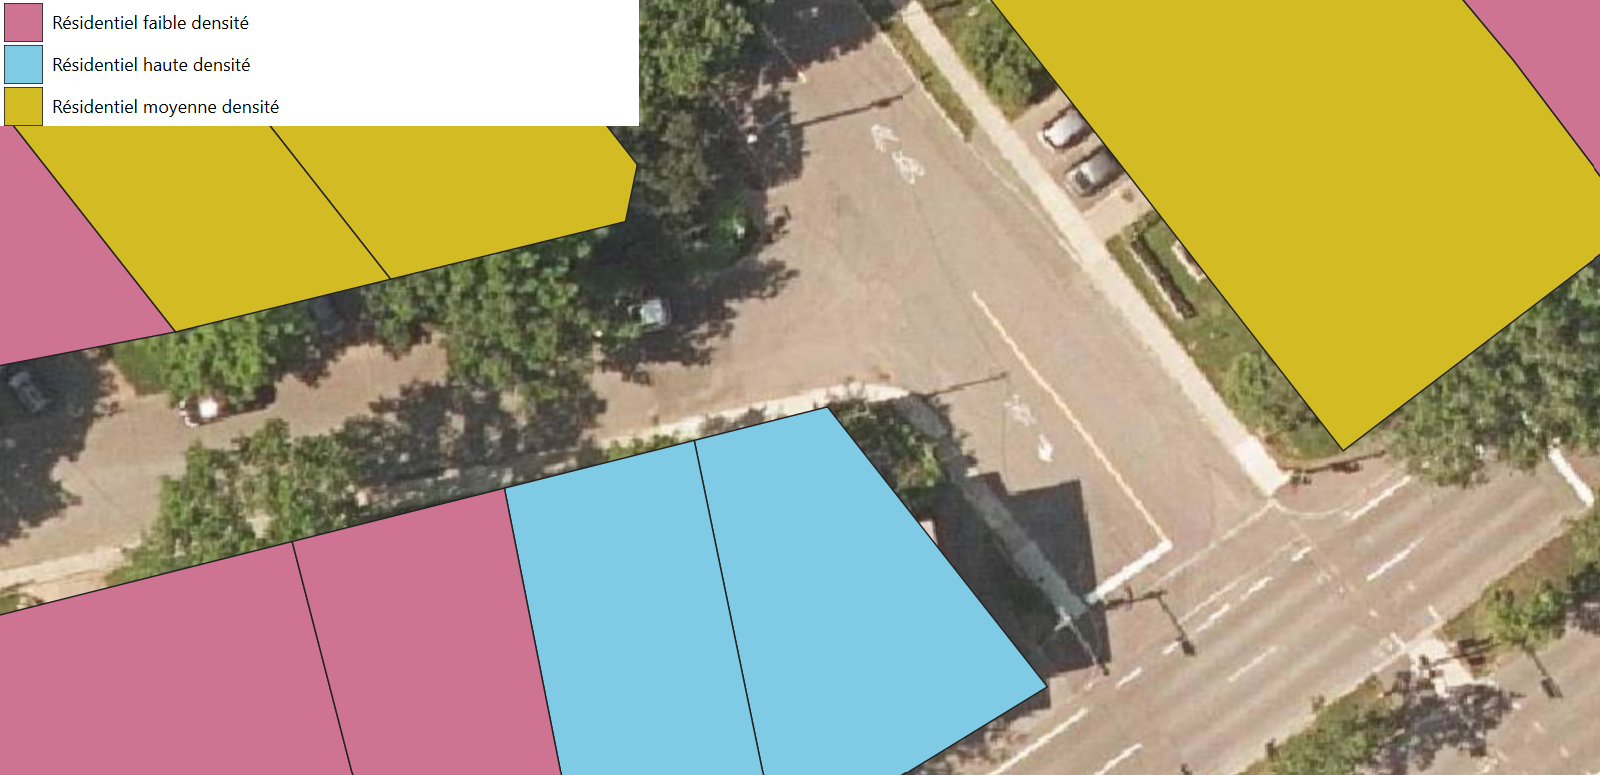
\includegraphics[width=1.0\textwidth]{images/utilisation_sols_Laurier_v2.png}
        \caption{Données polygonales disponibles}
        \label{fig:donnes_polygone_panneaux_Laurier}
        \end{subfigure}
        \caption{Données disponibles intersection Laurier}
      \end{figure}

      \FloatBarrier
    \subsubsection{Illustration - Cas 2: Coin de la Canardières - Desroches}
    Les figures \ref{fig:donnes_panneaux_Desroches} et \ref{fig:donnes_polygone_panneaux_Desroches} illustrent les mêmes données à un autre coin de rue. Ici, la localisation des panneaux porte encore plus à confusion puisque les panneaux de 2 tronçons de rue sont quasiment superposés. Il sera donc difficile d'assigner les panneaux aux bords de rues automatiquement lorsque ces derniers sont aux abords des intersections.
      \begin{figure}[ht]
        \centering
        \begin{subfigure}{\linewidth}
          \centering
          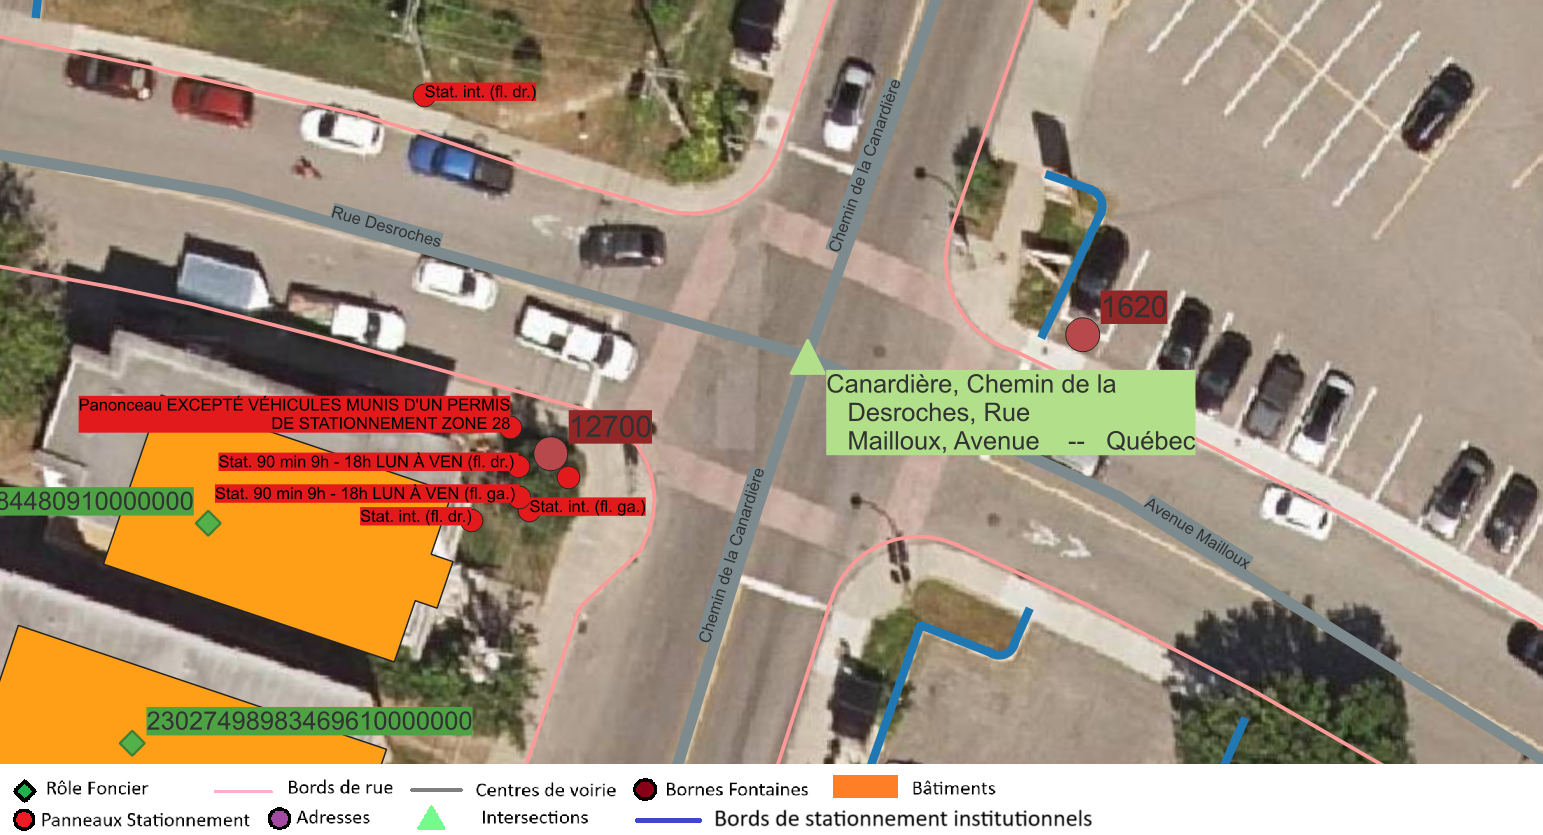
\includegraphics[width=0.8\textwidth]{images/donnees_disponible_Desroches_legende_v2.png}
        \caption{Données linéaires disponibles}
        \label{fig:donnes_panneaux_Desroches}
        \end{subfigure} \\
        \begin{subfigure}{\linewidth}
          \centering
          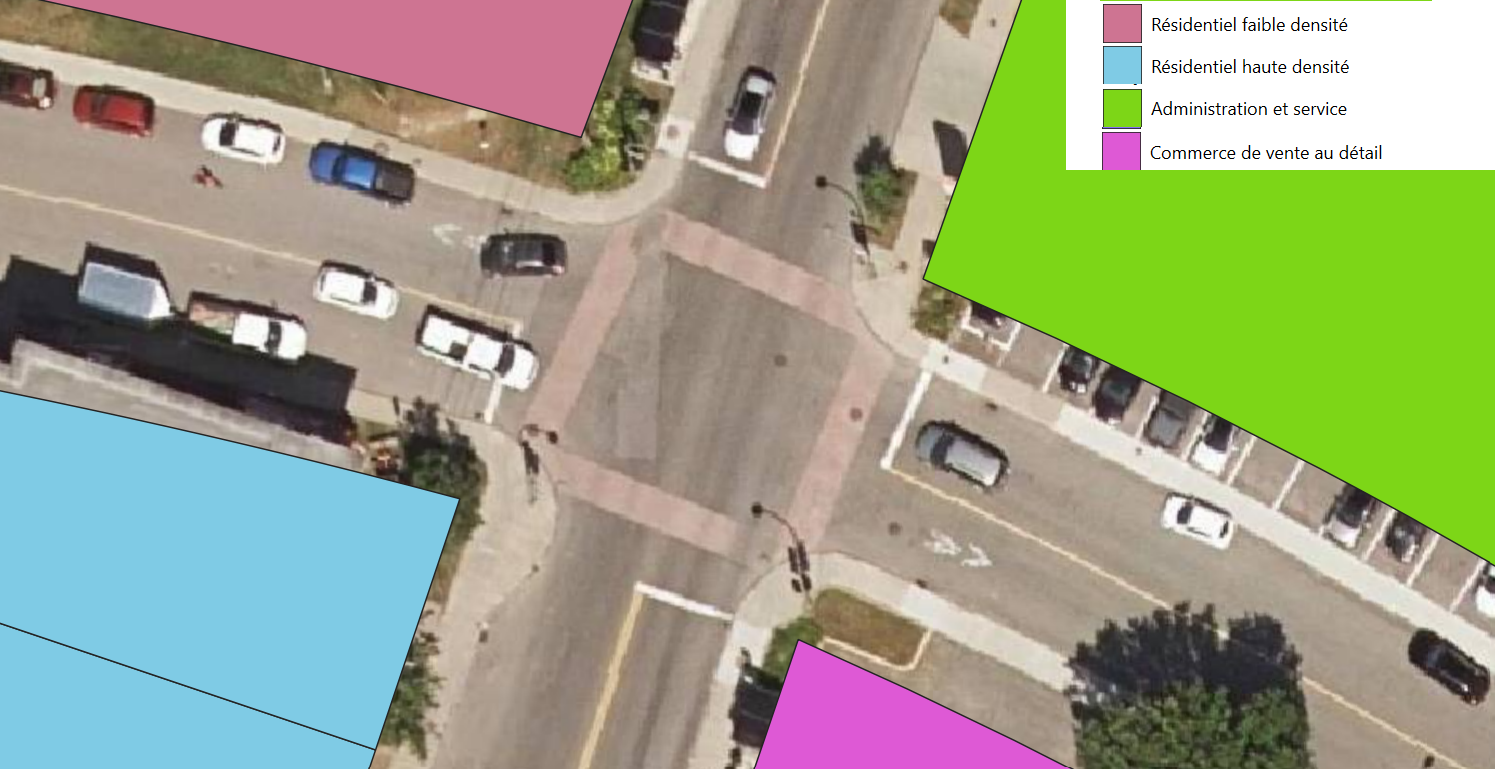
\includegraphics[width=0.8\textwidth]{images/utilisation_sols_Desroches_v2.png}
        \caption{Données polygonales disponibles}
        \label{fig:donnes_polygone_panneaux_Desroches}
        \end{subfigure}
        \caption{Données disponibles intersection Desroches / De la Canardière}
      \end{figure}
    
  \subsection{Entrainement d'apprentissage Machine}
    Plusieurs ensembles de données ont été créés pour la détection de places ouvertes dans un stationnement. Plus récemment, un ensemble de données annotées a été créé pour 
  \subsection{Enquête OD}
  \subsection{Imagerie Aérienne}
  \subsection{Rôle Foncier}
  \subsection{Recensement}
  
\section{Méthode d'inventaire sur rue}
  \subsection{Prétraitement des données}
    \subsubsection{Panneaux de stationnement}
      \subsubsection{Lisibilité Machine}
        Les panneaux ne sont pas classifiés de manière à être facilement lisibles par machine. Aucun index des panneaux de stationnement n'existe à la connaissance de l'auteur. Une classification semi-automatisée en isolant certains morceaux de chaînes de caractères a donc été créée pour rendre les panneaux de stationnement compatibles avec la structure de base de données énoncée dans \textcite{Bourdeau:MethodologieAnalyse:2014} et \textcite{Morency:DeveloppementMise:2022}. Le tableau \ref{tab:donnees_requises} liste les champs requis pour définir la fonction d'un panneau de stationnement:
        \LTcapwidth=\textwidth

        \begin{longtable}{p{0.15 \linewidth}  l p{0.5\linewidth} l  }
          \hline
          Champs & Type & Description & Valeur possibles \\
          \hline
          \endhead
          \hline
          \endfoot
          \hline
          \caption{Champs requis dans la base de données de stationnement}
          \label{tab:donnees_requises}
          \endlastfoot
          DUREE \_MAX\_ MINUTES & Entier & Durée maximale de stationnement & 0-120 \\
          TYPE\_1 & Entier & Clientèle spécifique de ce panneau & 0-11\\
          TYPE\_2 & Entier & Clientèle spécifique de ce panneau & 0-11\\
          ANNUEL & Booléen & Règlementation applicable à l'année & Vrai-Faux \\
          Date\_debut\_1 & Entier &  Date d'entrée en vigueur de la règlementation & 0-365\\
          Date\_fin\_1 & Entier & Date de fin de la règlementation & 0-365 \\
          Date\_debut\_2 & Entier & Date d'entrée en vigueur de la règlementation & 0-365 \\
          Date\_fin\_2 & Entier & Date de fin de la règlementation & 0-365 \\
          Q & Booléen & Règlementation applicable de manière quotidienne & Vrai - Faux \\
          Q\_d\_1 & Float & Heure d'entrée en vigueur de la règlementation & 0-24 \\
          Q\_f\_1 & Float & Heure de fin de la règlementation & 0-24\\
          Q\_d\_2 & Float & Heure de début de la deuxième période de validité de la règlementation 0-24\\
          LU & Booléen & Règlementation applicable un lundi (Q est nécessairement faux) & Vrai - Faux \\
          LU\_debut\_1 & Float & Heure d'entrée en vigueur de la règlementation & 0-24\\
          LU\_fin\_1 & Float & Heure d'arrêt de la règlementation & 0-24\\
          LU\_debut\_2 & Float & Deuxième Heure d'entrée en vigueur de la règlementation & 0-24\\
          LU\_fin\_2 & Float & Deuxième Heure d'arrêt de la règlementation & 0-24 \\
          MA & Booléen & Règlementation applicable un mardi (Q est nécessairement faux) & Vrai - Faux \\
          MA\_debut\_1 & Float & Heure d'entrée en vigueur de la règlementation & 0-24\\
          MA\_fin\_1 & Float & Heure d'arrêt de la règlementation & 0-24\\
          MA\_debut\_2 & Float & Deuxième Heure d'entrée en vigueur de la règlementation & 0-24\\
          MA\_fin\_2 & Float & Deuxième Heure d'arrêt de la règlementation & 0-24 \\
          ME & Booléen & Règlementation applicable un jeudi (Q est nécessairement faux) & Vrai - Faux \\
          ME\_debut\_1 & Float & Heure d'entrée en vigueur de la règlementation & 0-24\\
          ME\_fin\_1 & Float & Heure d'arrêt de la règlementation & 0-24\\
          ME\_debut\_2 & Float & Deuxième Heure d'entrée en vigueur de la règlementation & 0-24\\
          ME\_fin\_2 & Float & Deuxième Heure d'arrêt de la règlementation & 0-24 \\
          JE & Booléen & Règlementation applicable un jeudi (Q est nécessairement faux) & Vrai - Faux \\
          JE\_debut\_1 & Float & Heure d'entrée en vigueur de la règlementation & 0-24\\
          JE\_fin\_1 & Float & Heure d'arrêt de la règlementation & 0-24\\
          JE\_debut\_2 & Float & Deuxième Heure d'entrée en vigueur de la règlementation & 0-24\\
          JE\_fin\_2 & Float & Deuxième Heure d'arrêt de la règlementation & 0-24 \\
          VE & Booléen & Règlementation applicable un vendredi (Q est nécessairement faux) & Vrai - Faux\\
          VE\_debut\_1 & Float & Heure d'entrée en vigueur de la règlementation & 0-24\\
          VE\_fin\_1 & Float & Heure d'arrêt de la règlementation & 0-24\\
          VE\_debut\_2 & Float & Deuxième Heure d'entrée en vigueur de la règlementation & 0-24\\
          VE\_fin\_2 & Float & Deuxième Heure d'arrêt de la règlementation & 0-24 \\
          SA & Booléen & Règlementation applicable un samedi (Q est nécessairement faux) & Vrai - Faux \\
          SA\_debut\_1 & Float & Heure d'entrée en vigueur de la règlementation & 0-24\\
          SA\_fin\_1 & Float & Heure d'arrêt de la règlementation & 0-24\\
          SA\_debut\_2 & Float & Deuxième Heure d'entrée en vigueur de la règlementation & 0-24\\
          SA\_fin\_2 & Float & Deuxième Heure d'arrêt de la règlementation & 0-24 \\
          DI & Booléen & Règlementation applicable un samedi (Q est nécessairement faux) & Vrai - Faux \\
          DI\_debut\_1 & Float & Heure d'entrée en vigueur de la règlementation & 0-24\\
          DI\_fin\_1 & Float & Heure d'arrêt de la règlementation & 0-24\\
          DI\_debut\_2 & Float & Deuxième Heure d'entrée en vigueur de la règlementation & 0-24\\
          DI\_fin\_2 & Float & Deuxième Heure d'arrêt de la règlementation & 0-24 \\  
        \end{longtable}

      \FloatBarrier
      \subsubsection{Agrégation spatiale de plusieurs panneaux à un même endroit et association contextuelle}
    \subsubsection{Bords de rue}
    \subsubsection{Imagerie aérienne}
  \subsection{Conversion à une capacité de stationnement temporellement et spatiallement définie}
\section{Méthode d'inventaire hors rue basée sur les codes d'urbanisme}\label{sec:meth_urb_based_inventory}
    \subsection{Usages envisagés pour l'inventaire de stationnement}
    Plusieurs usages sont envisagés pour la base de données de stationnement. Il est important de les expliciter puisque cela sera la base pour l'établissement de requis pour la structure des données. Les usages envisagés sont donc les suivants:
    \begin{itemize}
        \item Étude d'accessibilité d'une place de stationnement à un lieu donnée (requiert que les places soient explicitées individuellement)
        \item Estimation du nombre de places de stationnement pour une destination précise
        \item Estimation du nombre de places de stationnement dans une zone d'analyse
        \item Analyse économétrique de l'effet de la tarification ou de la variation de l'offre sur les comportements de mobilité.
        \item Estimation de la surface minéralisée pour l'entreposage des voitures pour l'application d'écofiscalité   
    \end{itemize}
    Basé sur ces cas d'usage envisagés, la situation idéale serait d'avoir une base de données complètement désagrégée qui liste chaque place de stationnement. A minima, l'information doit être disponible au niveau du lot cadastral. D'autre part, il doit être possible d'encoder les informations relatives à la tarification de l'espace, le nombre disponible par lot , pour permettre d'appliquer des mesures d'écofiscalité. Il doit être possible d'agréger ces mesures au niveau à des zones d'analyse de déplacement pour faire des analyses sur la capacité de stationnement dans une zone dans un modèle de transport. \par
    Ultimement, l'ensemble de ces requis soulève la nécessité d'une base de donnée personnalisée. En effet, dans le cas d'un inventaire basé sur la règlementation, \ac{OSM} est mal adapté puisqu'il requiert la localisation précise des places ce qui n'est pas nécessairement faisable. D'autre part, cela ne lie pas le stationnement à un identifiant qui permet à une entité gouvernementale d'appliquer cette fiscalité. Idéalement, la base de données serait capable d'exporter un format importable dans \ac{OSM} pour mettre à jour les données ouvertes au public.
    \subsection{Choix d'une unité d'inventaire}
    Idéalement, il serait possible d'avoir la localisation précise de chaque place de stationnement. Cela permettrait de déterminer l'accessibilité aux destinations pour divers niveaux d'achalandage et choix de stationnement. Il est aussi nécessaire que les places soient agrégées par lot cadastral pour que les municipalités puissent appliquer des mesures d'écofiscalité et distribuer les places de stationnement aux divers comptes de taxes sur un même lot. Finalement, l'utilisation du lot cadastral est pertinente comme unité d'agrégation puisque que les requis sont souvent applicables à un lot qui à la construction aura des usages relativement bien définis. L
    \subsection{Proposition de base de données}
    La figure \ref{fig:offstreet_db_erd} montre la structure de la base de données utilisée pour l'estimation de l'offre de stationnement. 
    \begin{landscape}
    \begin{figure}
        \centering
        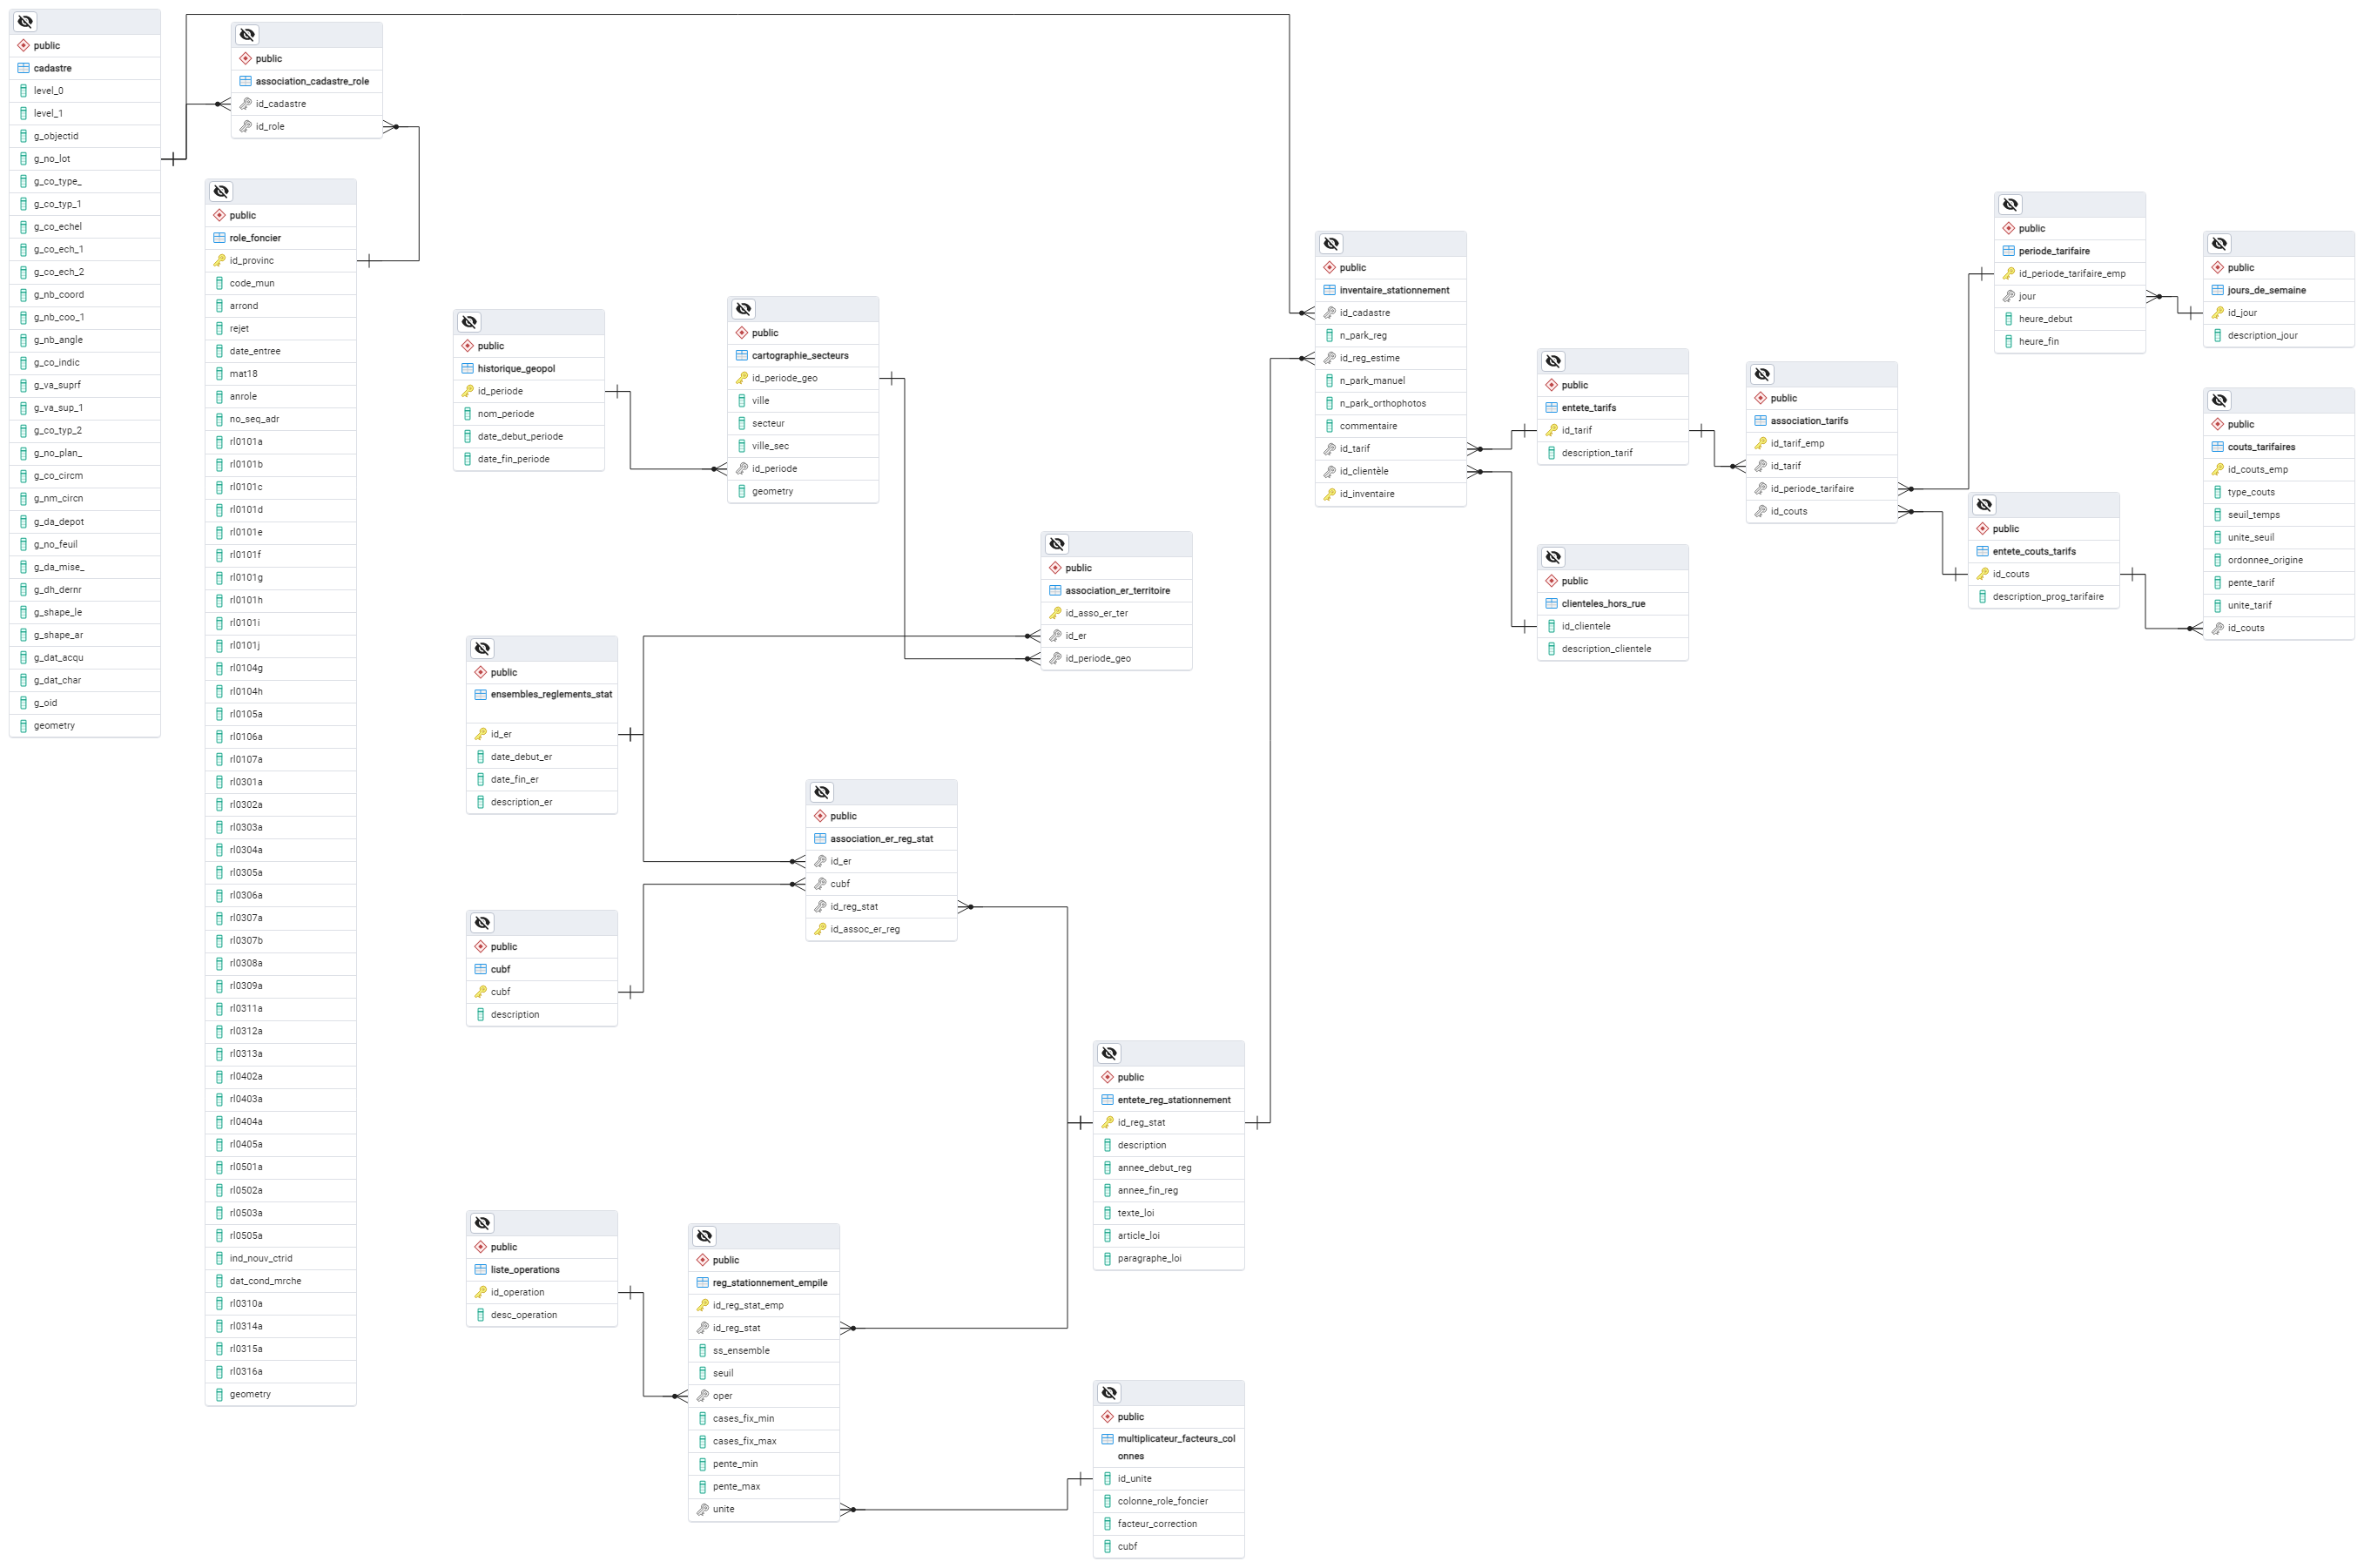
\includegraphics[width = 0.85\linewidth]{images/structure_base_de_donnee.png}
        \caption{Diagramme entité association de la base de données}\label{fig:offstreet_db_erd}
    \end{figure}
    \end{landscape}
    La base de données est implémentée dans PostgreSQL avec PostGIS pour pouvoir gérer les données spatiales du rôle foncier, du cadastre ainsi que de la division géopolitique du territoire.\par
    
    \subsubsection{Données sortantes}
    La table \underline{inventaire\_stationnement} contient l'inventaire de stationnement. La table laisse la possibilité d'avoir plusieurs estimations par lot cadastral. Ainsi, l'usager peut utiliser une estimation règlementaire, entrer une valeur manuellement ou utiliser une méthode d'estimation basée sur les orthophotos. D'autre part, des identifiants de clientèle et de tarif sont mis en place. On pourrait ainsi avoir un cas où sur un même lot cadastral il y a plusieurs stationnements (par exemple, employés, résidents, clients de commerces) ayant des modalités d'accès différentes. Chaque stationnement aurait alors un identifiant de clientèle et un identifiant de tarif. Une clé primaire est mise en place pour chaque stationnement sous la forme de la colonne id\_inventaire. Le champ id\_reg\_estime permet d'identifier le règlement d'urbanisme utilisé pour définir l'offre de stationnement estimée basé sur les règlements d'urbanisme. Cette valeur correspond à id\_reg\_stat dans la table entete\_reg\_stationnement qui sera présentée à la prochaine section.\par
    La table \underline{entete\_tarifs} est la table contenant une description et une clé primaire d'identifiant de tarifs vers laquelle pointe la table d’inventaire. La table \underline{association\_tarifs} joint une période tarifaire, un tarif et l'identifiant de tarif. La table \underline{periode\_tarifaire} permet de définir des périodes de validité. Chaque période tarifaire a un identifiant unique, un identifiant de jours, une heure de début et une heure de fin. \par
    Les tarifs ont chacun un entête avec un identifiant et une description entreposés dans la table \underline{entete\_couts\_tarifs}. La table \underline{couts\_tarifaires} contient les données de tarification. La structure a été ainsi faite pour permettre plusieurs types de tarification en fonction de l'heure de la journée et une progression de la tarification. Les champs de la table sont type\_couts qui définit s'il s'agit d'un abonnement un paiement à l'entrée ou un paiement en sortie. Le champ seuil\_temps et unite\_seuil définissent un seuil au-delà duquel le tarif s'applique. Les champs ordonnee\_origine, pente\_tarif, unite\_tarif définissent l'ordonnée à l'origine, la pente et l'unité à fournir entrée pour obtenir le prix du stationnement.\par
    Pour conclure, la table \underline{clienteles\_hors\_rue} définit l'association entre le type de clientèle et l'entier enregistré dans la table \underline{inventaire\_stationnement}. Les valeurs possibles envisagées sont listées au tableau \ref{tab:clienteles_hors_rue}.
    \begin{table}
    \centering
    \begin{tabular}{l l}
    \hline
    id\_clientèle & Description clientèle\\ \hline
    0& Automobiles - Propriétaire et Visiteurs Autorisés \\
    1 & Automobiles - Propriétaires Seulement \\
    2 & Automobiles - Clients \\
    3 & Automobiles - Employés seulement \\
    4 & Automobiles - Véhicules autorisés \\
    5 & Automobiles - Vignettes résidents \\
    6 & Automobiles - Vignettes Autres \\
    7 & Automobiles - Tous\\ \hline
    \end{tabular}
    \caption{Entrées dans la table \underline{clienteles\_hors\_rue}}\label{tab:clienteles_hors_rue}
    \end{table}
    \FloatBarrier
    La figure \ref{fig:offstreet_db_erd_output} montre le détail de la base de données discutée dans cette section. Cette structure permet de séparer les places disponibles aux différentes clientèles de manière extensible pour chaque lot et de répertorier des structures de tarification complexe au besoin.
    \begin{figure}[!h]
        \centering
        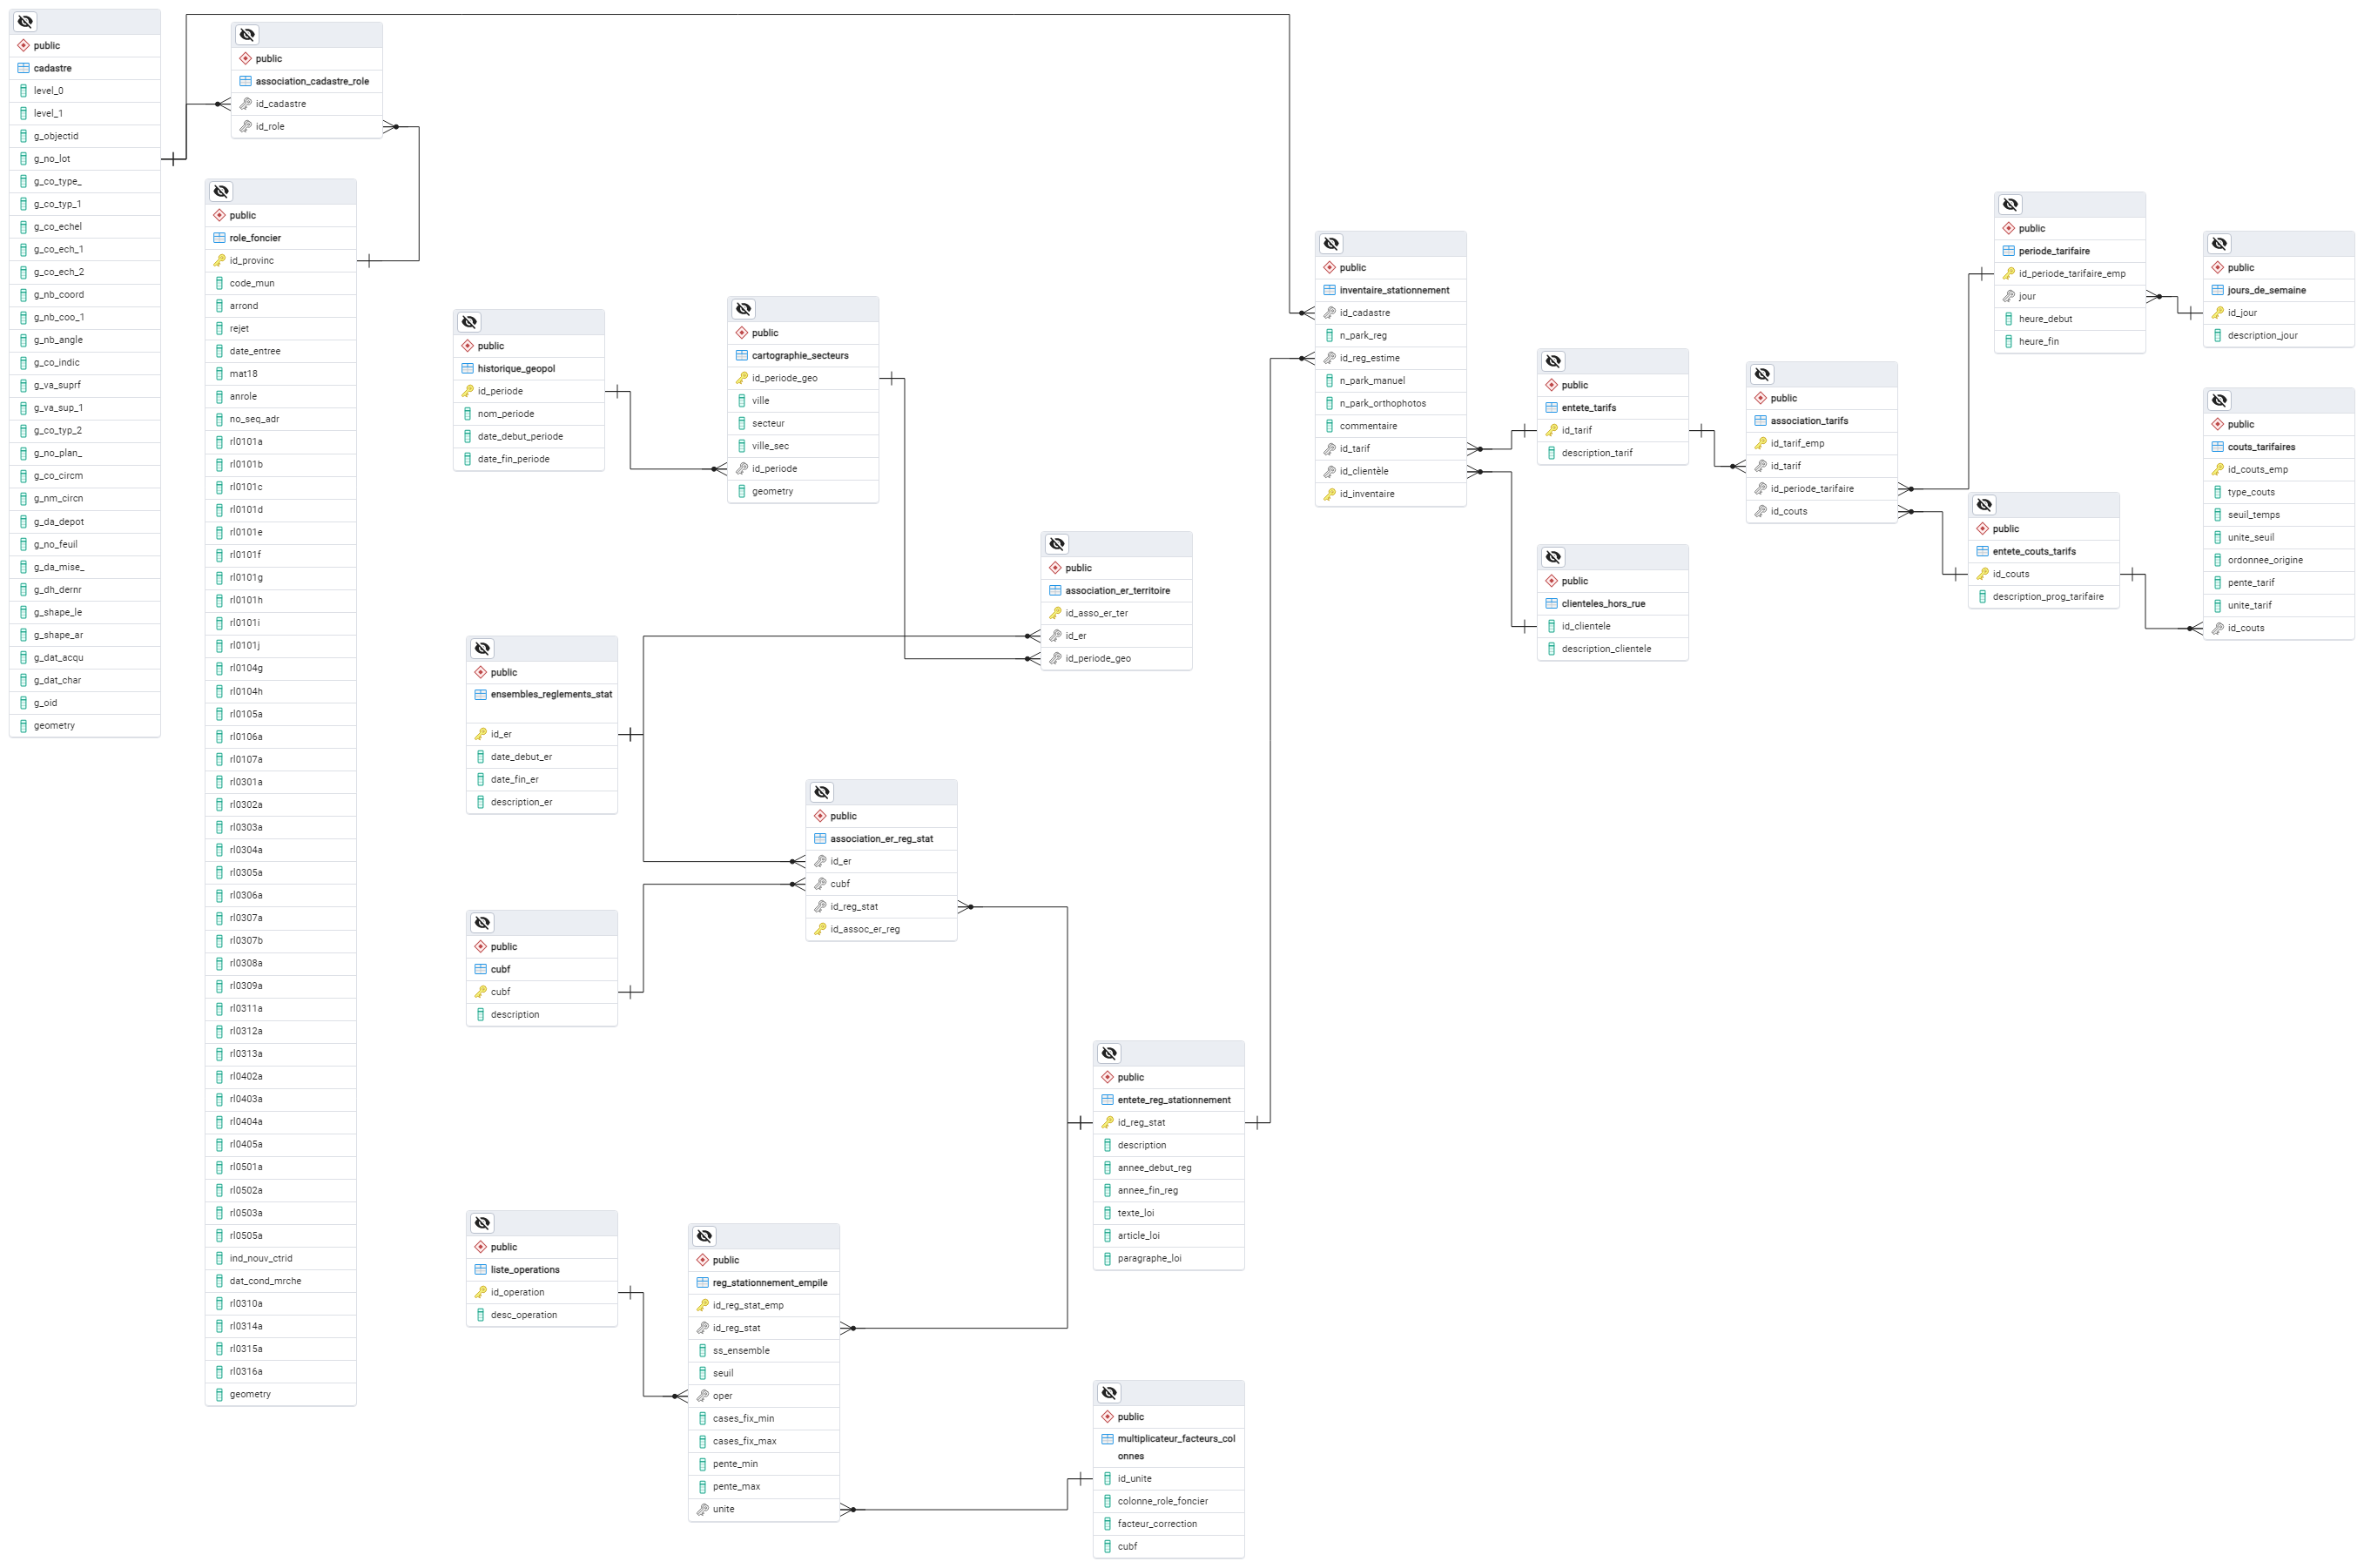
\includegraphics[trim={50cm 35cm 0 7cm}, clip, width=14cm]{images/structure_base_de_donnee.png}
        \caption{Structure de données en sortie de procédure de calcul}\label{fig:offstreet_db_erd_output}
    \end{figure}
    \FloatBarrier

    
    \subsubsection{Représentation des limites géopolitiques au travers du temps} 
    Une composante de la méthodologie proposée est d'utiliser les règlements d'urbanisme pour proposée une estimation de la capacité de stationnement basé sur les règlements d'urbanisme. Cette section présentera la manière dont la règlementation est représentée dans la base de données.
    \paragraph{Historique géopolitique} L'historique géo politique de la ville est représenté au moyen de deux tables: \underline{historique\_geopol} et \underline{cartographie\_secteurs}. \underline{historique\_geopol} représente les grandes périodes où le territoire a été stable. Dans le cadre de ce mémoire, 6 grandes périodes ont été identifiées basé sur \textcite{VilledeQuebec:ReperesChronologique:} et \textcite{ElectionsQuebec:AtlasHistorique:2021}. Elles sont listées au tableau \ref{tab:histo_geopol}
    \begin{table}
    \centering
    \begin{tabular}{c p{5cm} c c}
    \hline
    \makecell{Identifiant\\ id\_periode} & \makecell[l]{Nom \\ nom\_periode} & \makecell{Année début \\ date\_debut\_periode} & \makecell{Année fin \\ date\_fin\_periode}\\ \hline
    1 & Fondation - 1970 &  S.V. & 1970 \\
    3 & Duberger, Saules et Neufchâtel fusion Québec & 1971 & 1975 \\
    4 & Fusions Charlesbourg & 1976 & 1994 \\
    5 & Inauguration VQZ-3 & 1995 & 1996 \\
    6 & Abrogation Zone Prioritaire Ville de Québec & 1997 & 2009 \\
    7 & Harmonisation & 2010 & S.V.\\ \hline
    \end{tabular}
    \caption{Valeurs dans l'historique géopolitique utilisé dans le cadre de ce mémoire}\label{tab:histo_geopol}
    \end{table}
    \FloatBarrier
    La table \underline{cartographie\_secteurs} contient les délimitations des secteurs pour chacune des périodes. Les champs sont les suivants :id\_periode\_geo est l'identifiant primaire, id\_periode est la clé qui référence à la table \underline{historique\_geopol}, le champ ville contient le nom de la ville, le champ secteur est un nom de secteur, et le champ ville\_sec est une concaténation des deux champs précédents. En plus de l'information tabulaire, les limites géographiques des secteurs sont entreposées dans cette table. \par
    La figure \ref{fig:offstreet_db_erd_history} montre le détail de la section de base de donnée montrant l'évolution des variations géopolitiques du territoire.
    \begin{figure}
        \centering
        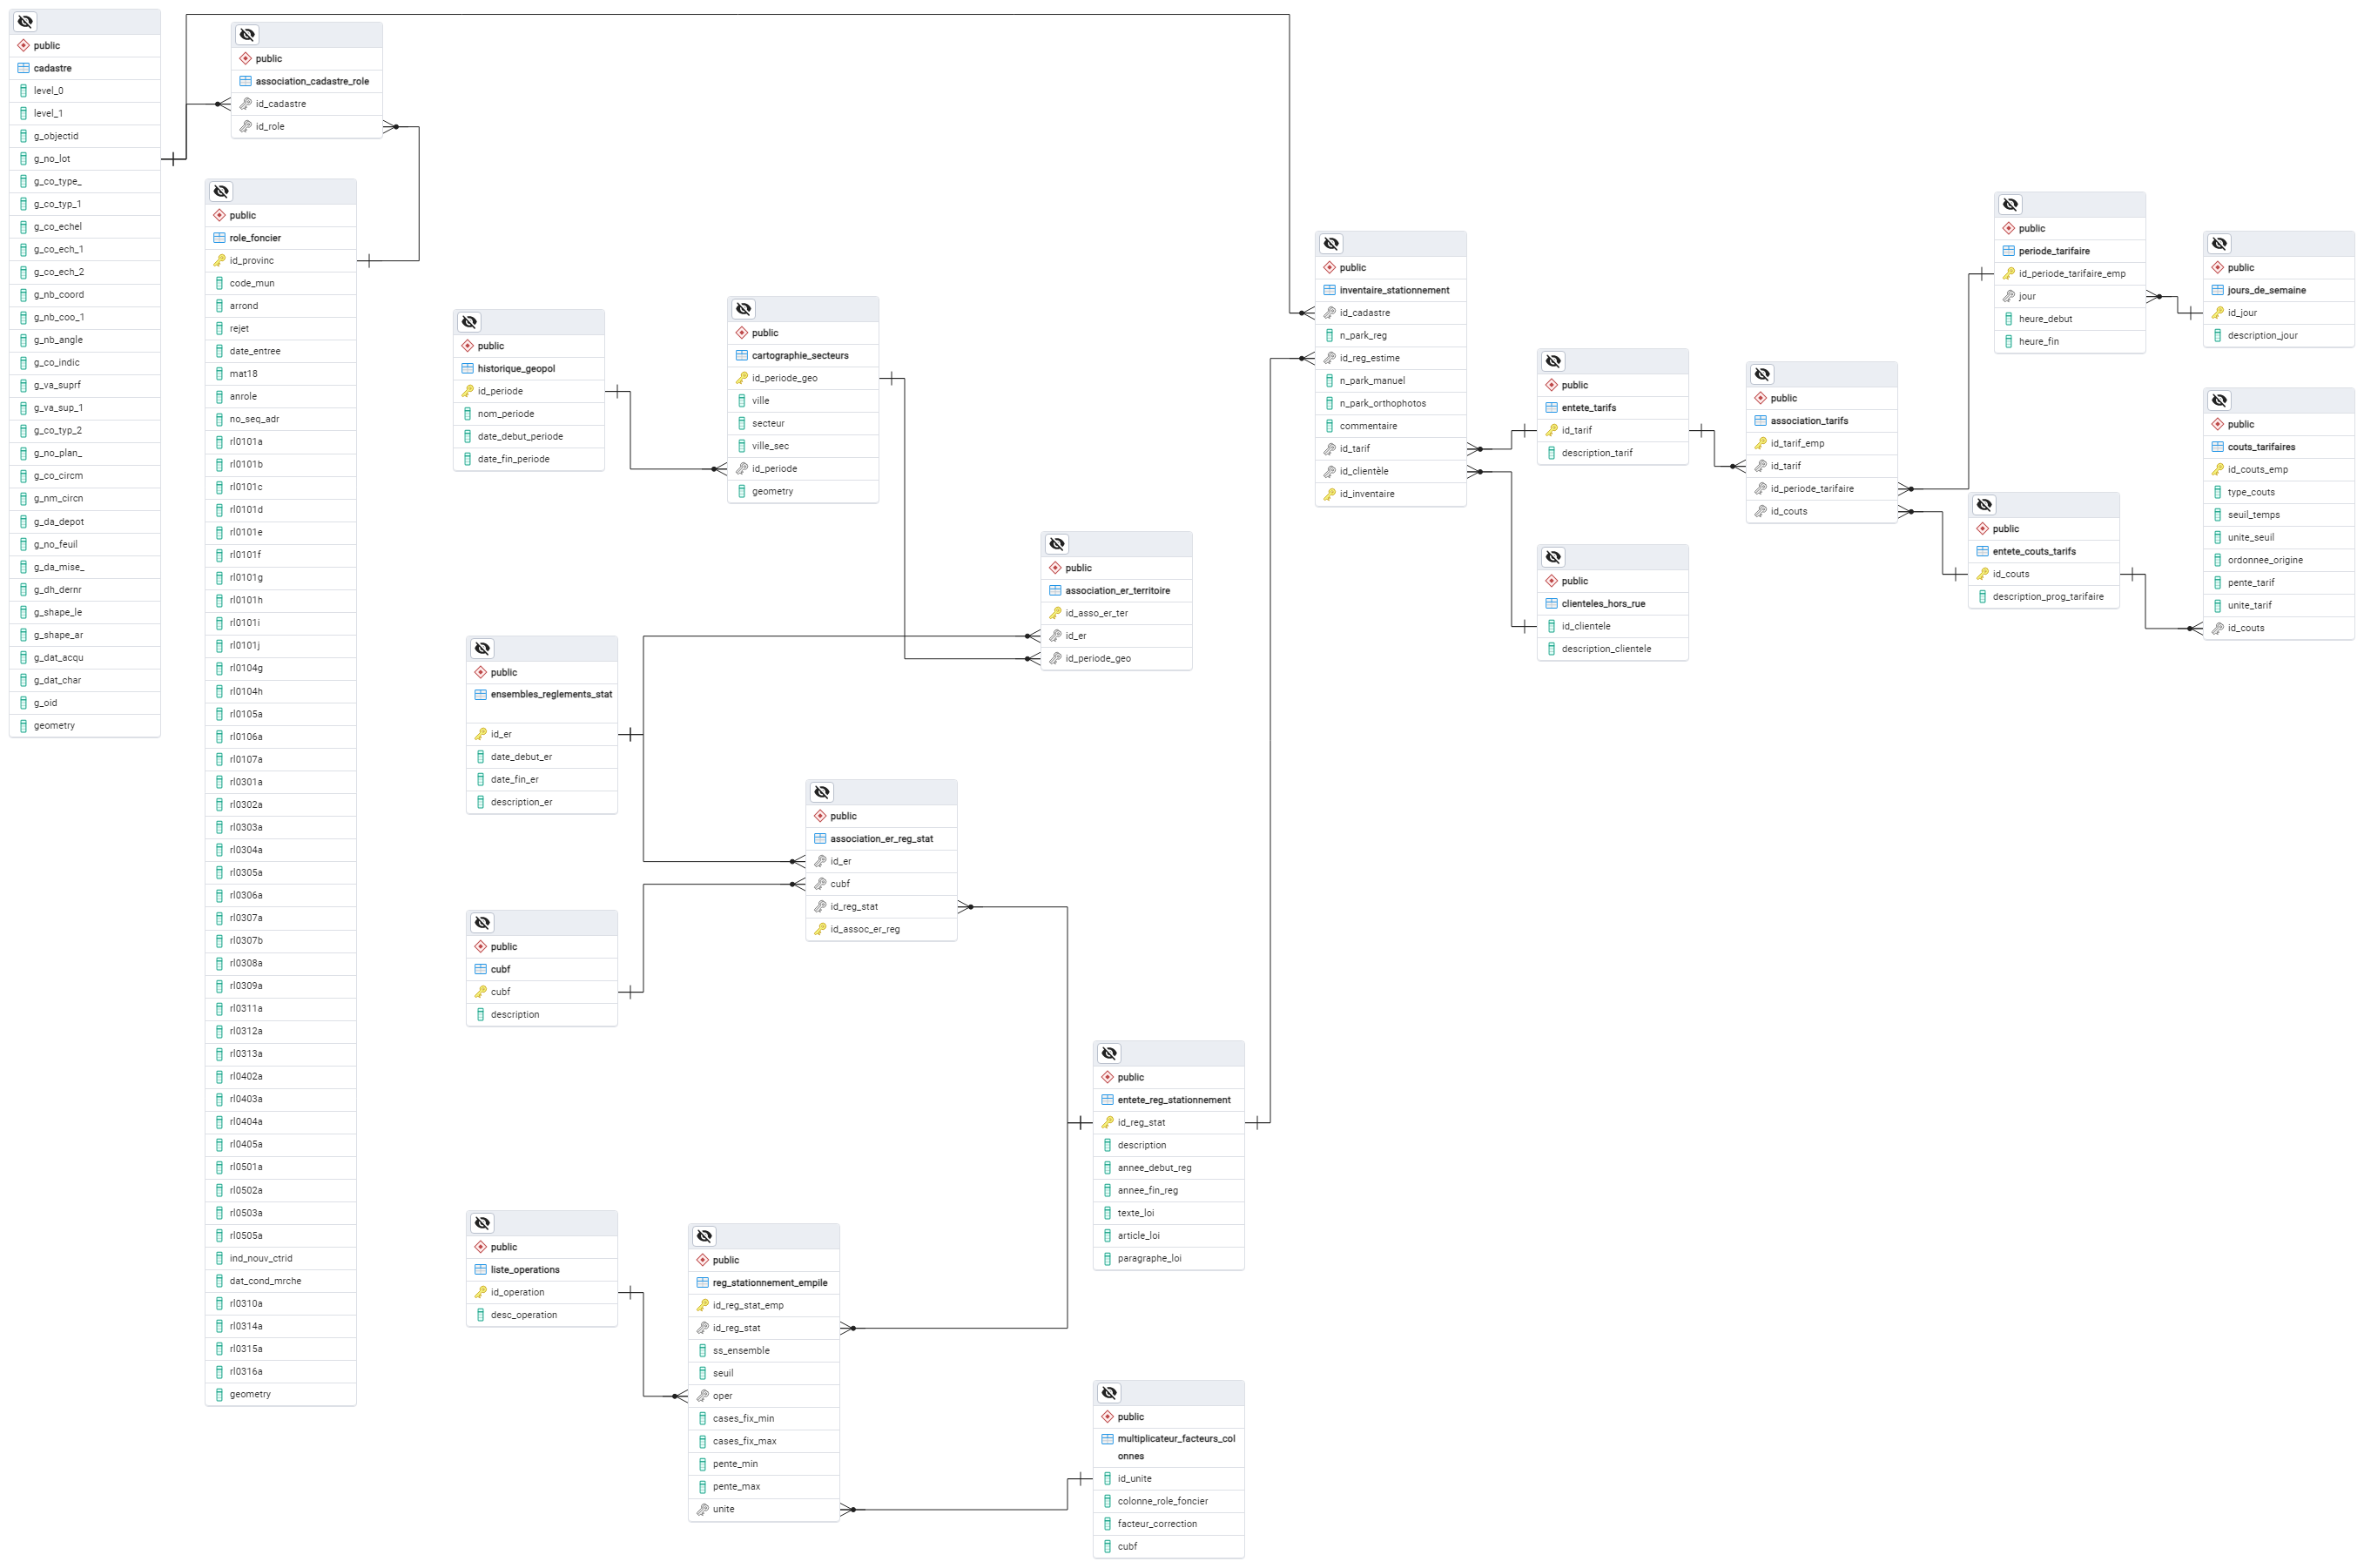
\includegraphics[trim={18cm 40cm 60cm 12cm}, clip, width=8cm]{images/structure_base_de_donnee.png}
        \caption{Structure de données pour l'historique géopolitique}\label{fig:offstreet_db_erd_history}
    \end{figure}
    \FloatBarrier
    
    \subsubsection{Représentation de règlements individuels} 
    Les règlements sont ensuite définis individuellement dans la table \underline{entete\_reg\_stationnement}. Cette table contient les champs suivants: id\_reg\_stat est l'identifiant unique pour chaque règlement, le champ description est une description textuelle issue du règlement décrivant l'usage du sol associé au règlement, annee\_debut\_reg contient la date d'entrée en vigueur du règlement, annee\_fin\_reg contient l'année d'abrogation du règlement, texte\_loi, article\_loi et paragraphe\_loi contiennent la provenance du règlement et ville indique la ville qui a issue le règlement. La description du nombre de places requises est entreposée dans la table \underline{reg\_stat\_empile}. Les champs de la table sont les suivants: id\_reg\_stat\_emp est l'identifiant unique pour la table, id\_reg\_stat permet d'unifier plusieurs lignes de la table à un même règlement. Cette stratégie permet de représenter des règlements complexes sur plusieurs lignes de la base de données. La colonne ss\_ensemble permet de définir des sous-ensembles au règlement, ce champ permet de séparer des conditions complexes.  Le champ seuil définit une borne inférieure à son applicabilité. L'unité pour le seuil est la même que celle utilisée en entrée des équations linéaires définies dans les autres champs de la même ligne. Le champ oper contient l'opération à appliquer à la ligne. Toutes les lignes sauf la première devraient avoir une valeur pour ce champ. Les champs cases\_fix\_min et cases\_fix\_max définissent l'abscisse à l'ordonnée, pente\_min et pente\_max définissent la pente, et unite définit l'unité utilisée. Le champ unité et un entier et est la clé primaire pour la table \underline{multiplicateur\_facteurs\_colonnes}. \par 
    Les opérations possibles sont listées dans la table liste\_operations qui a deux champs: id\_operation et desc\_operation. Les valeurs possibles sont listées au tableau \ref{tab:operations_table}.
    \begin{table}[h]
        \centering
        \begin{tabular}{cl}
             \hline
             id\_operation & desc\_operation  \\ \hline
             1 & + (absolu)\\
             2 & + (au-delà seuil >=)(obsolète)\\
             3 & ou (plus contraignant) \\
             4 & changement critère au dela seuil (>=)\\
             5 & changement critère dans centre commercial(obsolète)\\
             6 & ou simple \\ \hline
        \end{tabular}
        \caption{Opérations listées dans la table liste\_operations}
        \label{tab:operations_table}
    \end{table}
    Cette dernière contient trois 5 champs: id\_unite, colonne\_role\_foncier, facteur\_correction, cubf, desc\_unite. Le champ id\_unite est référencé par le champ unite de la table \underline{reg\_stat\_empile}, colonne role foncier donne le nom de la colonne dans le rôle foncier qui doit être utilisée dans l'équation et la comparaison au seuil, la colonne facteur correction donne la possibilité de multiplier la valeur dans la colonne du rôle foncier pour appliquer une correction. Le champ cubf permet de donner un facteur de correction différent pour différents types de \ac{CUBF}. Le champ desc\_unite donne une brève description de l'unité. Le tableau \ref{tab:unite_pertinentes_minimum_stat} donne les le contenu de la table multiplicateur\_facteur\_colonnes.\par
    \begin{table}[h]
    \centering
        \begin{tabular}{c l c c p{3cm}}
            \hline
            id\_unite & colonne\_role\_foncier & facteur\_correction & cubf & desc\_unite \\ \hline
            1 & rl0312a & 1 & S.V. & chambre\\
            2 & rl0311a & 1 & S.V. & logement \\
            4 & rl0308a & 1 & S.V. & metre carré d'étage\\
            5 & S.V. & 1 & S.V. & metre carré bureau\\
            6 & S.V. & 1 & S.V. & metre carré salle production \\
            7 & rl0302a & 1 & S.V. & metre carré terrain\\
            8 & S.V. & 1 & S.V. & siège \\
            9 & S.V. & 1 & S.V. & poste de travail \\
            10 &S.V. & 1 & S.V. & salle \\
            11 & S.V. & 1 & S.V. & lit \\
            12 & S.V. & 1 & S.V. & personne \\
            13 & S.V. & 1 & S.V. & employé \\
            14 & S.V. & 1 & S.V. & étudiant \\
            15 & S.V. & 1 & S.V. & médecin \\
            16 & S.V. & 1 & S.V. & quai \\
            17 & S.V. & 1 & S.V. & voie de service \\
            18 & S.V. & 1 & S.V. & vert \\
            19 & S.V. & 1 & S.V. & allee de pratique \\
            20 & S.V. & 1 & S.V. & plateau sportif \\ \hline
        \end{tabular}
        \caption{Unités utilisées pour codifier les codes d'urbanismes}\label{tab:unite_pertinentes_minimum_stat}
    \end{table}
    \FloatBarrier
    Les équations donnent les étapes mathématiques pour une ligne d'un règlement de stationnement sont donc données aux équations \ref{eq:x_entree}, \ref{eq:places_max} et \ref{eq:places_min} si $x_{entree} \geq seuil $.
    \begin{align}
        x_{entree} &= role\_foncier[colonne\_role\_foncier] \times facteur\_correction \label{eq:x_entree}\\
        n_{places,min} &= cases\_fix\_min + pente\_min \times x_{entree} \label{eq:places_min}\\
        n_{places,max} &= cases\_fix\_max + pente\_max \times x_{entree} \label{eq:places_max}
    \end{align}
    \clearpage
    \paragraph{Exemple 1: Clinique medicale} Admettons un règlement qui requiert 1 place par salle de consultation  plus une place par employé plus une place par médecin ou une place par 20 mètres carrés, au plus contraignant. Les entrées dans la table reg\_stat\_empile seraient telles que montrées au tableau \ref{tab:ex_reg_stat_clinique}
    \begin{table}[h]
        \centering
        \begin{tabular}{cccccccccc}
            \hline
            \rotatebox{90}{id\_emp} & \rotatebox{90}{id\_reg\_stat} & \rotatebox{90}{ss\_ensemble} & \rotatebox{90}{seuil}  & \rotatebox{90}{oper}  & \rotatebox{90}{cases\_fix\_min}   & \rotatebox{90}{cases\_fix\_max}   & \rotatebox{90}{pente\_min}    & \rotatebox{90}{pente\_max} & \rotatebox{90}{unite}    \\ \hline
            1                       & 1                             &  1                           & 0                      &  S.V.                 & 0                                 & S.V.                              & 1                             & S.V.                       & 15                       \\
            2                       & 1                             &  1                           & 0                      &  1                    & 0                                 & S.V.                              & 1                             & S.V.                       & 13                       \\
            3                       & 1                             &  1                           & 0                      &  1                    & 0                                 & S.V.                              & 1                             & S.V.                       & 10                       \\
            4                       & 1                             &  2                           & 0                      &  3                    & 0                                 & S.V.                              & 0.05                          & S.V.                       & 4                       \\ \hline
        \end{tabular}
        \caption{Exemple règlements dans la table reg\_stat\_empile pour une clinique médicale}
        \label{tab:ex_reg_stat_clinique}
    \end{table}
    \begin{figure}[h]
    \begin{subfigure}[t]{0.5\textwidth}
       \centering
       \begin{tikzpicture}[scale=0.8]
        \begin{axis}[
            xlabel={$N_{employes}$[-]},
            ylabel={$N_{médecin}$[-]},
            zlabel={$N_{places}$[-]},
            legend style={at={(0.5,1.25)},
	           anchor=north,legend columns=-1}
        ]
        \addplot3[
            surf,color = blue, faceted color=black,
        ] 
        coordinates {
        (0,0,1) (0,1,2) (0,2,3)
        
        (1,0,2) (1,1,3) (1,2,4)
        
        (2,0,3) (2,1,4) (2,2,5)
        };
        \addplot3[
            surf,color = orange, faceted color=black,
        ] 
        coordinates {
        (0,0,2) (0,1,3) (0,2,4)
        
        (1,0,3) (1,1,4) (1,2,5)
        
        (2,0,4) (2,1,5) (2,2,6)
        };
        \legend{Stat min. $n_{salles}=1$,Stat min. $n_{salles}=2$}
        \end{axis} 
        \end{tikzpicture}
        \caption{Sous ensemble 1 du règlement}
    \end{subfigure}
    ~
    \begin{subfigure}[t]{0.5\textwidth}
        \centering
        \begin{tikzpicture}[scale = 0.9]
        \begin{axis}[
            xlabel={Espace de plancher [$m^2$]},
            ylabel={$N_{places}$[-]},
            xmin=0, xmax=200,
            ymin=0, ymax=10,
            xtick={0,100,200},
            ytick={0,5,10},
                legend pos=north west,
            ymajorgrids=true,
            xmajorgrids=true,
            grid style=dashed,
            domain=0:1000, 
        ]
        \addplot[color=blue]{x/20};
        \legend{Stationnement min}
        \end{axis}
    \end{tikzpicture}
    \caption{Sous ensemble 2 du règlement}
    \end{subfigure}
    \caption{Exemple de règlement de stationnement pour une clinique médicale}
    \end{figure}
    \FloatBarrier
    \clearpage
    \paragraph{Exemple 2: Logements} Dans le cas d'un logement, les règlements changes souvent en fonction du nombre de logements au sein d'un même bâtiment. Dans ce cas hypothétique, le requis serait de une case par logement pour des bâtiments de moins de 4 logements, 1.5 cases par logement pour les bâtiments entre 4 et 7 logements et 1.25 case par logements pour tout bâtiment de 8 logements ou plus. Dans ce cas, les entrées à la table seraient telles que montrées au tableau
    \begin{table}[h]
        \centering
        \begin{tabular}{cccccccccc}
            \hline
            \rotatebox{90}{id\_emp} & \rotatebox{90}{id\_reg\_stat} & \rotatebox{90}{ss\_ensemble} & \rotatebox{90}{seuil}  & \rotatebox{90}{oper}  & \rotatebox{90}{cases\_fix\_min}   & \rotatebox{90}{cases\_fix\_max}   & \rotatebox{90}{pente\_min}    & \rotatebox{90}{pente\_max} & \rotatebox{90}{unite}    \\ \hline
            5                       & 2                             &  1                           & 0                      &  S.V.                 & 0                                 & S.V.                              & 1                             & S.V.                       & 2                       \\
            6                       & 2                             &  1                           & 4                      &  4                    & 0                                 & S.V.                              & 1.5                           & S.V.                       & 2                       \\
            7                       & 2                             &  1                           & 8&  4                    & 0                                 & S.V.                              & 1.25                          & S.V.                       & 2                       \\ \hline
        \end{tabular}
        \caption{Exemple règlements dans la table reg\_stat\_empile pour le logement}
        \label{tab:ex_reg_logement}
    \end{table}
     \begin{figure}[h]
       \centering
        \begin{tikzpicture}[scale=1.0]
            \begin{axis}[
                xlabel={$N_{logements}$[-]},
                ylabel={$N_{places}$[-]},
                xmin=0, xmax=20,
                ymin=0, ymax=30,
                xtick={0,5,10,15,20},
                ytick={0,5,10,15,20,30},
                legend pos=north west,
                ymajorgrids=true,
                grid style=dashed,
            ]
            \addplot[
                    color=blue
                    ]
                 coordinates {
                    (0,0)(3,3)(4,6)(5,7.5)(6,9)(7,10.5)(8,10)(10,12.5)(15,18.75)(20,25)
                };
    
            \legend{Stationnement min}
            \end{axis}
        \end{tikzpicture}
    \caption{Exemple de règle de stationnement pour logement}
    \end{figure}
    \FloatBarrier
    \clearpage
    \paragraph{Exemple 3: Lieux d'assemblée} Dans le cas de lieux d'assemblée, les requis peuvent être exprimés en fonction du nombre de sièges ou en fonction de l'espace au sol. Dans notre cas hypothétique, le requis serait un minimum d'une place par 7 sièges jusqu'à 800 sièges et d'un minimum de 1 place par 9 sièges pour toute place au-delà de 800 siège. Un maximum  d'une place par 5 sièges est applicable au-delà de 500 sièges. Quand il n'y a pas de sièges, un requis d'une places par 10 mètres carrés est applicable sans maximum.
    \begin{table}[h]
        \centering
        \begin{tabular}{cccccccccc}
            \hline
            \rotatebox{90}{id\_emp} & \rotatebox{90}{id\_reg\_stat} & \rotatebox{90}{ss\_ensemble} & \rotatebox{90}{seuil}  & \rotatebox{90}{oper}  & \rotatebox{90}{cases\_fix\_min}   & \rotatebox{90}{cases\_fix\_max}   & \rotatebox{90}{pente\_min}    & \rotatebox{90}{pente\_max} & \rotatebox{90}{unite}    \\ \hline
            8                       & 3                             &  1                           & 0                      &  S.V.                 & 0                                 & S.V.                              & 0.142857                      & S.V.                       & 8                       \\
            9                       & 3                             &  1                           & 500                    &  4                    & 0                                 & 0                                 & 0.142857                      & 0.2                        & 8                       \\
            10                      & 3                             &  1                           & 800                    &  4                    & 25.396825                         & 0                                 & 0.111111                      & 0.2                        & 8                       \\
            11                      & 3                             &  2                           & 0                      &  6                    & 0                                 & S.V.                              & 0.1                           & S.V.                       & 4                       \\\hline
        \end{tabular}
        \caption{Exemple règlements dans la table reg\_stat\_empile pour un lieu d'assemblée}
        \label{tab:ex_reg_lieu_assemblee}
    \end{table}
   \begin{figure}[h]
        \begin{subfigure}[t]{0.5\textwidth}
        \centering
            \begin{tikzpicture}[scale = 0.9]
            \begin{axis}[
                xlabel={$N_{sièges}$[-]},
                ylabel={$N_{places}$[-]},
                xmin=0, xmax=1000,
                ymin=0, ymax=200,
                xtick={0,200,400,600,800,1000},
                ytick={0,50,100,150,200},
                    legend pos=north west,
                ymajorgrids=true,
                grid style=dashed,
            ]
        
            \addplot[
                color=blue
                ]
            coordinates {
            (0,0)(500,71.4285)(800,114.2856)(1000,136.507938)
            };
            \addplot[
            color = red
            ]
            coordinates{
                (500,100)(1000,200)
            };
            \legend{Stationnement min, Stationnement max}
            \end{axis}
        \end{tikzpicture}
            \caption{Avec sièges}
    \end{subfigure}
    \begin{subfigure}[t]{0.5\textwidth}
        \centering
        \begin{tikzpicture}[scale = 0.9]
        \begin{axis}[
            xlabel={Espace de plancher [$m^2$]},
            ylabel={Nombres de places[-]},
            xmin=0, xmax=1000,
            ymin=0, ymax=200,
            xtick={0,200,400,600,800,1000},
            ytick={0,50,100,150,200},
                legend pos=north west,
            ymajorgrids=true,
            grid style=dashed,
        ]
        \addplot[
            color=blue
            ]
        coordinates {
        (0,0)(500,50)(800,80)(1000,100)
        };
        \legend{Stationnement min}
        \end{axis}
    \end{tikzpicture}
        \caption{Sans sièges}
    \end{subfigure}
    \captionsetup{justification=centering}
\caption{Exemple de règle de stationnement pour lieux d'assemblée}
\end{figure}
    \FloatBarrier
    \subsubsection{Création d'ensembles de règlements}
    Du fait de la variation de la règlementation dans le temps, des règlements instaurés à différents moments peuvent être applicables à une même période. Pour permettre de créer un tout cohérent représentant l'état de la règlementation à un instant T à un endroit sur le territoire de l'actuelle ville de Québec. Cette section va introduire le schéma relationnel de ces ensembles de règlements. Trois tables sont crées pour assurer l'expansibilité du système: \underline{ensembles\_reglements\_stat}, \underline{cubf}, \underline{association\_er\_reg\_stat}.\par
    \underline{ensembles\_reglements\_stat} a 4 colonnes: id\_er est un identifiant unique pour chaque ensemble de règlements, description\_er est une description textuelle de chaque ensemble de règlements, date\_debut\_er et date\_fin\_er décrivent les années de validité de l'ensemble de règlements.\par
    \underline{cubf} contient le numéro et la description de chaque \acf{CUBF}.\par
    \underline{association\_er\_reg\_stat} permet de faire l'association entre les \ac{CUBF}, les ensembles de règlements et les règlements décrits à la section précédente. Cette table est constituée de 4 colonnes: id\_er qui est l'indice de l'ensemble de règlements pour lequel on fait l'association, cubf qui dit pour quelle utilisation du territoire on assigne un règlement de stationnement, id\_reg\_stat qui indique quel règlement défini à la section précédente on associe au cubf et id\_assoc\_er\_reg qui est la clé primaire de la table.\par
    La figure \ref{fig:offstreet_db_erd_rulesets} montre les tables de la base de données qui permettent de définir un ensemble de règlements.
    \begin{figure}[h]
        \centering
        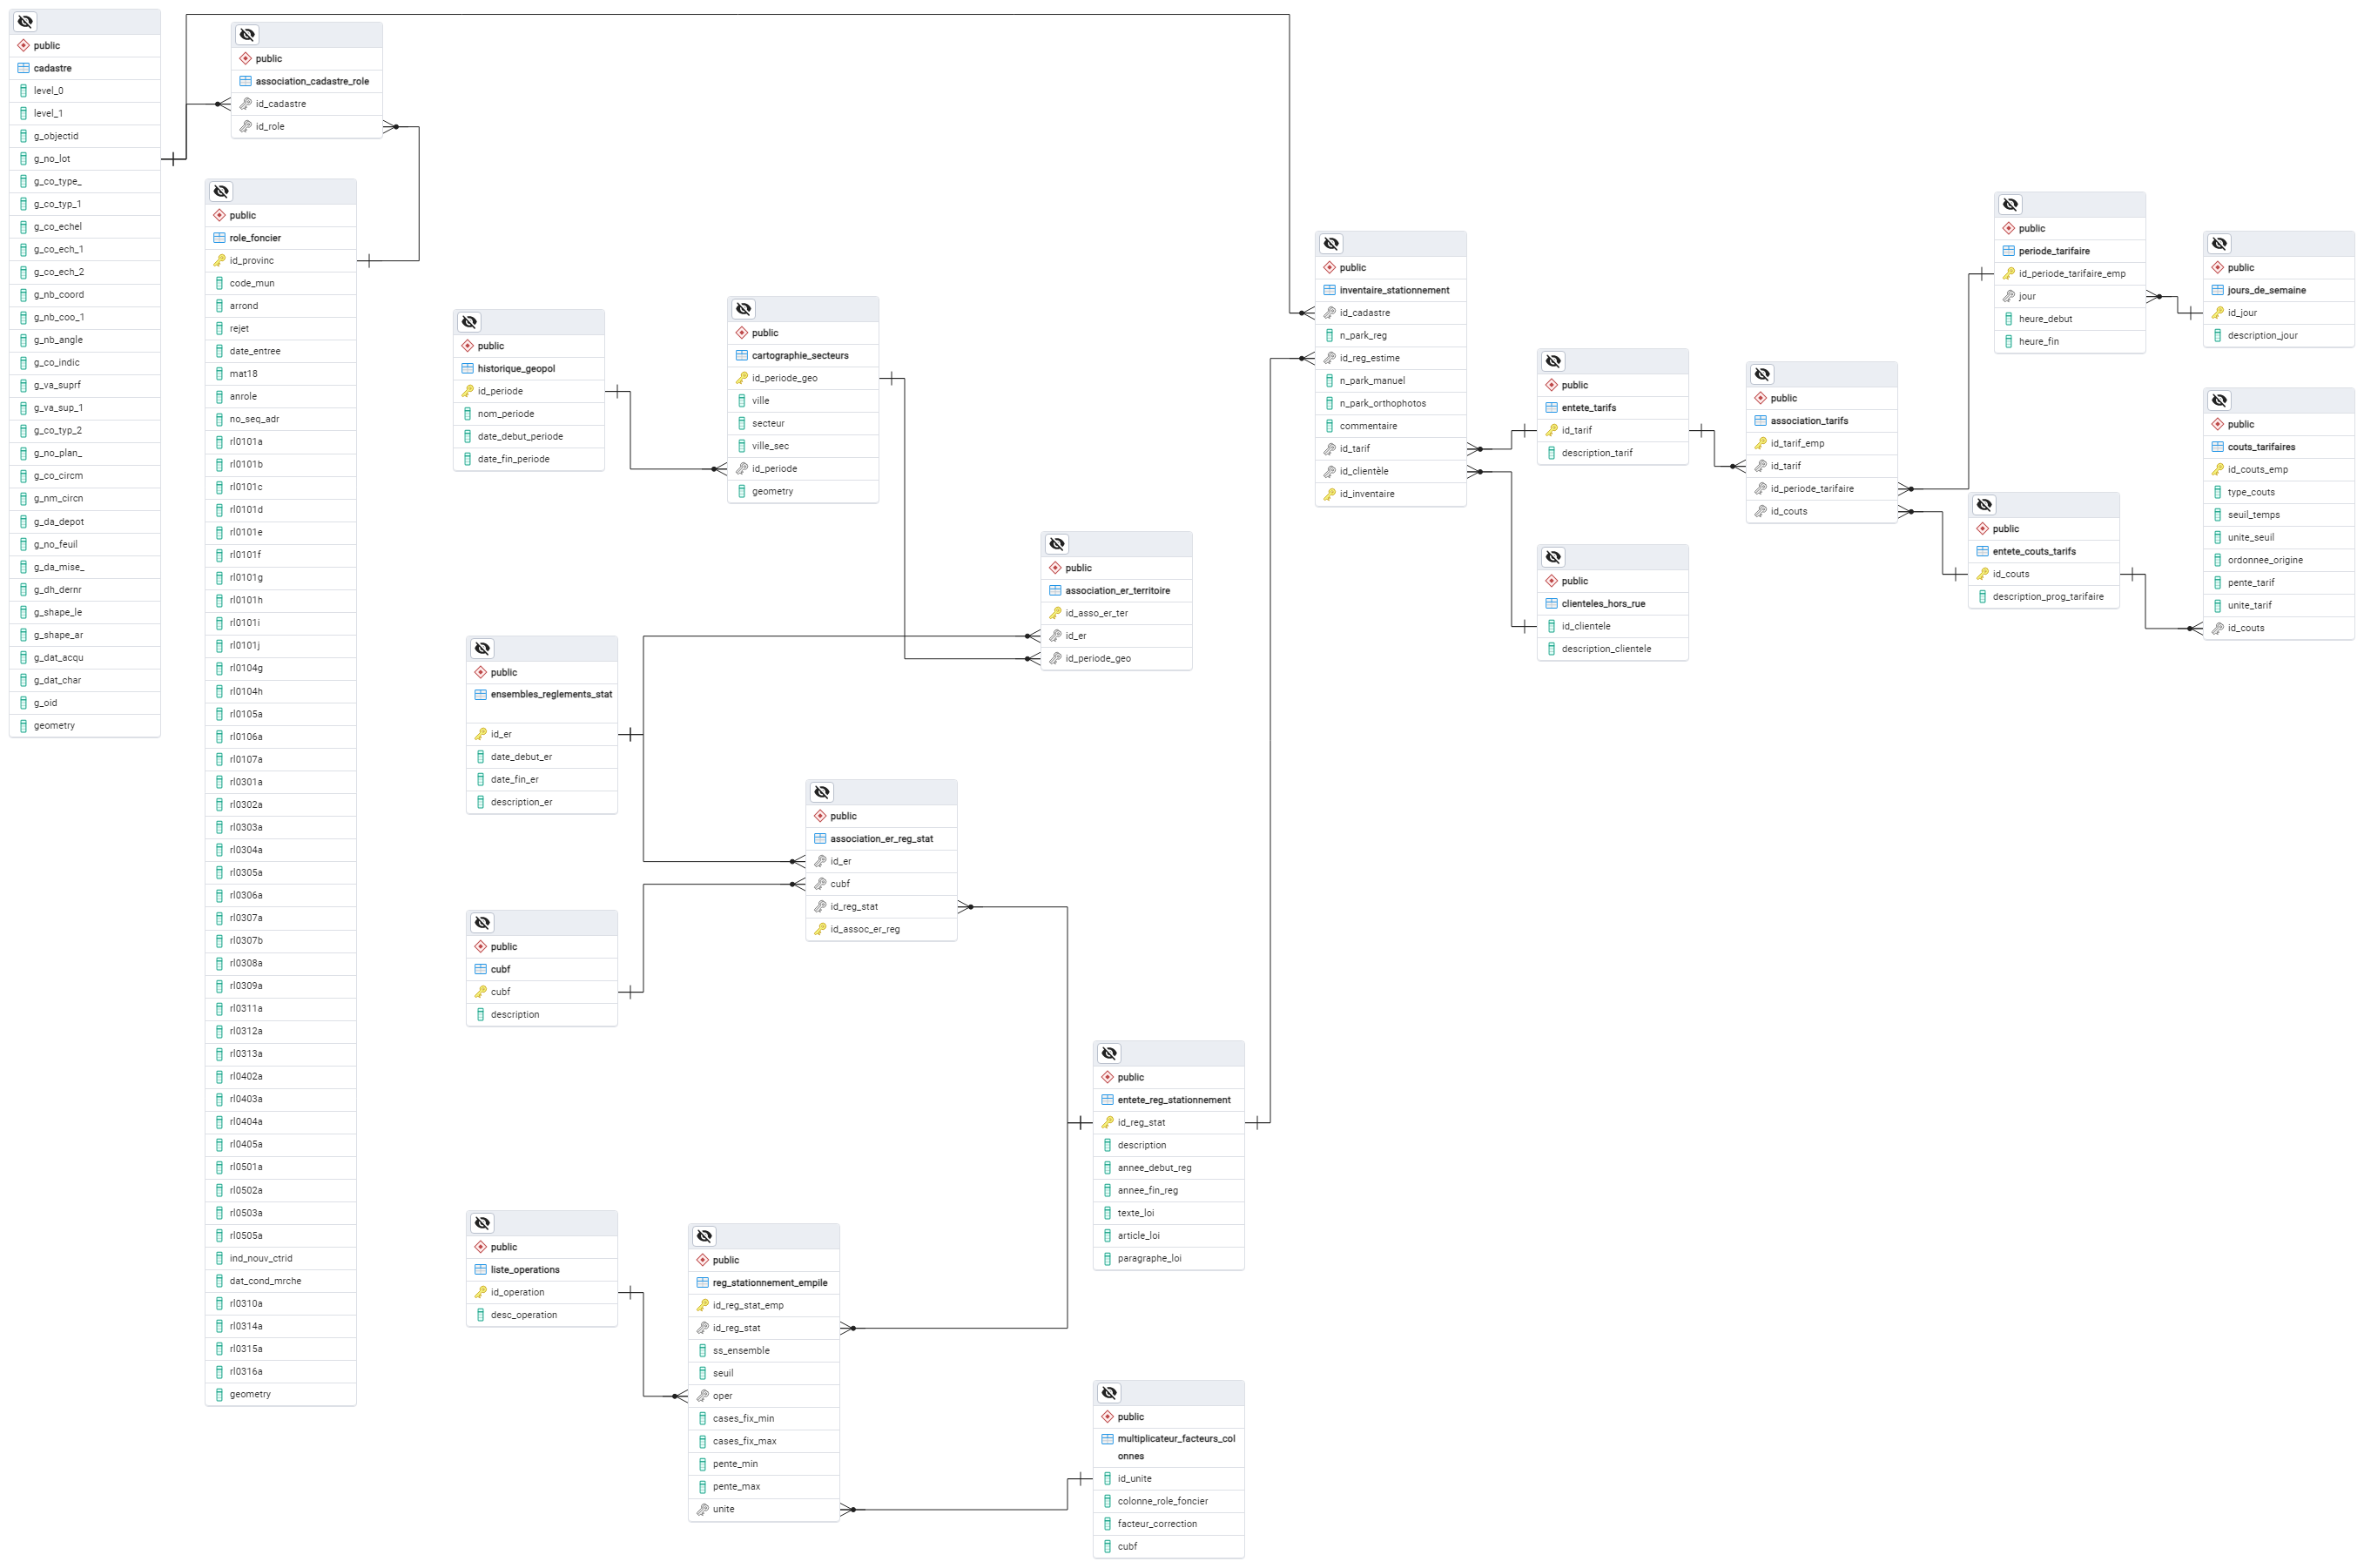
\includegraphics[trim={16cm 22cm 55cm 24cm},clip,width=12.5cm]{images/structure_base_de_donnee.png}
        \caption{Schéma relationnel pour la définition d'ensembles de règlements}
        \label{fig:offstreet_db_erd_rulesets}
    \end{figure}
    \FloatBarrier

    
    \subsubsection{Association du territoire aux ensembles de règlements}
    La table \underline{association\_er\_territoire} est nécessaire pour associer les territoires aux ensembles de règlements. Elle comporte trois champs: id\_asso\_er\_ter qui est la cle primaire, id\_er qui fait référence à la clé primaire de \underline{ensembles\_reglements\_stat} et id\_periode\_geo qui fait référence à la clé primaire de \underline{cartographie\_secteurs}. La figure \ref{fig:offstreet_db_erd_er_ter} montre les champs de la table.
    \begin{figure}[h]
        \centering
        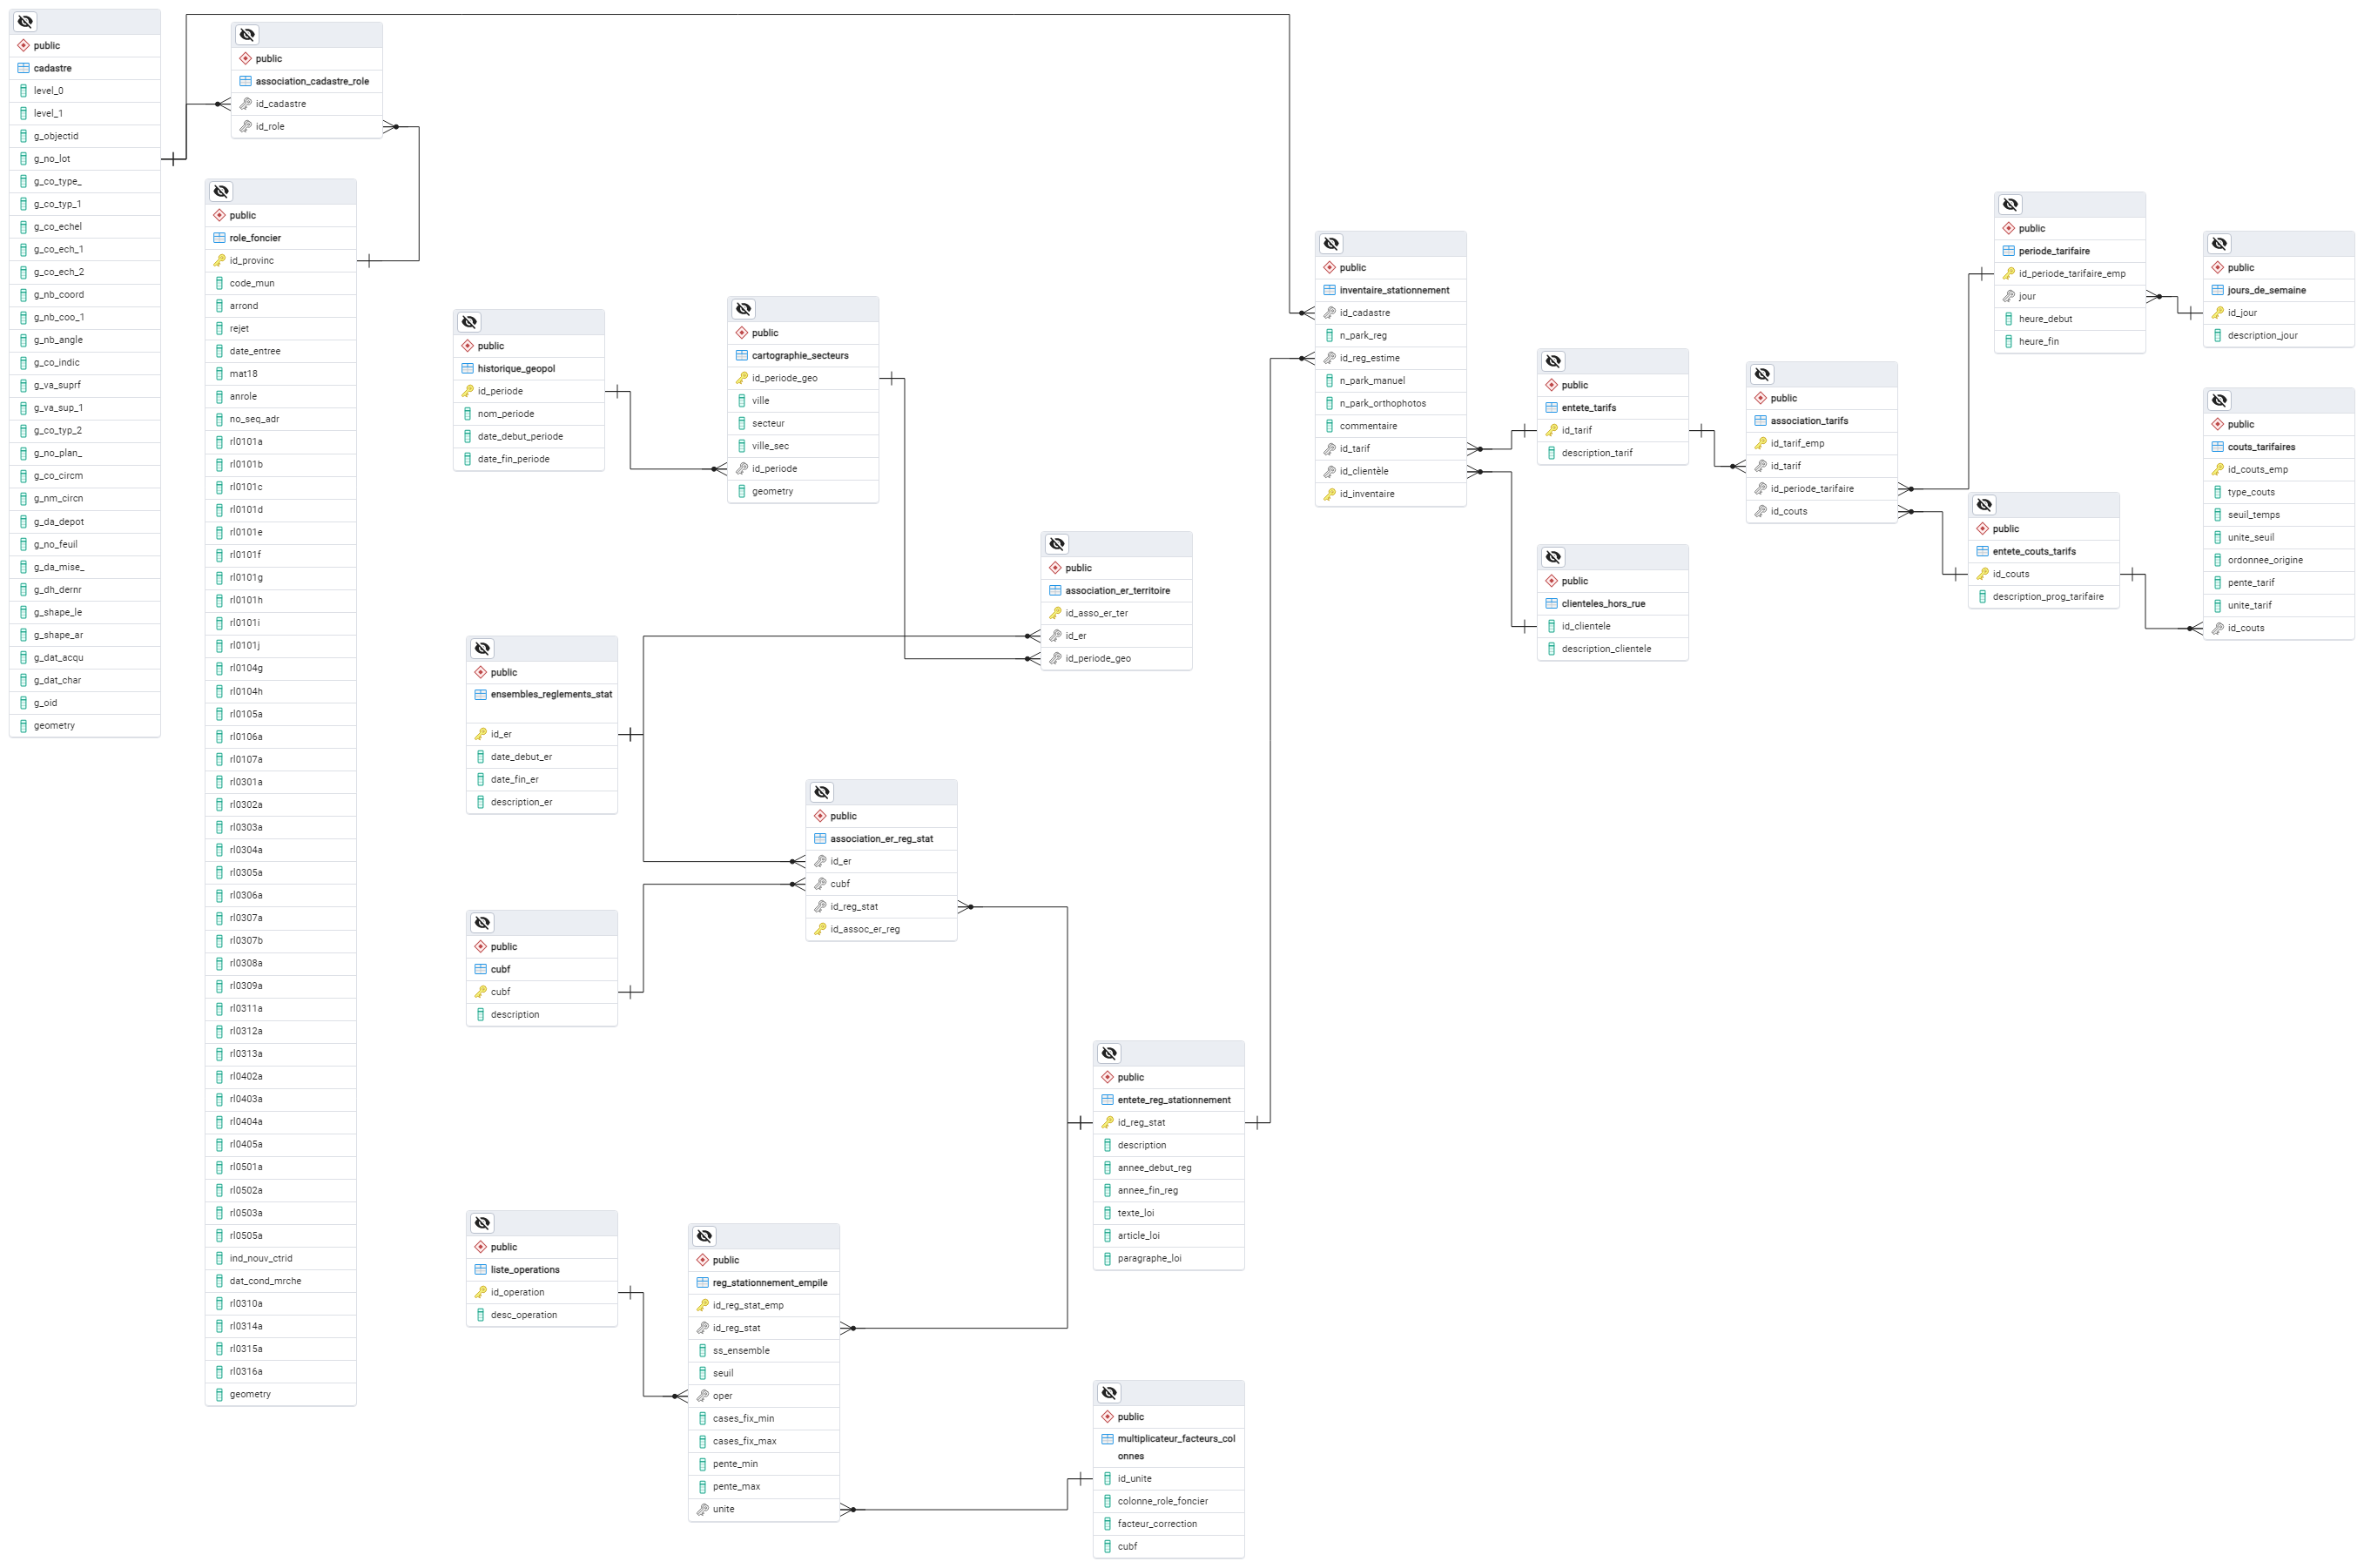
\includegraphics[trim={28cm 25cm 55cm 30cm},clip,width=5cm]{images/structure_base_de_donnee.png}
        \caption{Schéma relationnel pour l'association des règlements aux territoires}
        \label{fig:offstreet_db_erd_er_ter}
    \end{figure}
    \FloatBarrier

    
    \subsubsection{Données de départ}Les données de départ sont le rôle foncier brut ainsi que le cadastre représentés dans les tables \underline{cadastre} et \underline{role\_foncier}. Inclus dans ces tables sont l'ensemble des champs qui proviennent des données disponibles sur Géo-Index et Données Québec. \par
    Le cadastre est utilisé pour pouvoir améliorer la cartographie et la représentation des données sur une carte choroplèthe. La table \underline{association\_cadastre\_role} associe le cadastre avec le rôle foncier. En théorie, une jointure géométrique pourrait être complétée, mais celle-ci peut être onéreuse et mener à des erreurs pour des lots avec des formes concaves. L'approche faisant l'association dans une table permet de gérer ces formes sans manipulation une fois une première correction complétée. Ceci est différent de l'approche utilisée par la chaire, où les points du cadastre sur l'entrée principale du bâtiment. L'approche proposée ici permet d'utiliser les données brutes du cadastre qui sont issues de \textcite{GouvernementduQuebec:ManuelEvaluation:2024}. Clé primaire pour le cadastre est g\_no\_lot et la clé primaire pour le rôle est l'id\_provinc.\par
    La figure \ref{fig:offstreet_db_erd_input_data} montre les tables pertinentes en intrant. Il est concevable que ces tables soient entreposés dans un serveur différent si cette méthodologie était implémenté dans un milieu municipal.
    \begin{figure}[ht!]
        \centering
        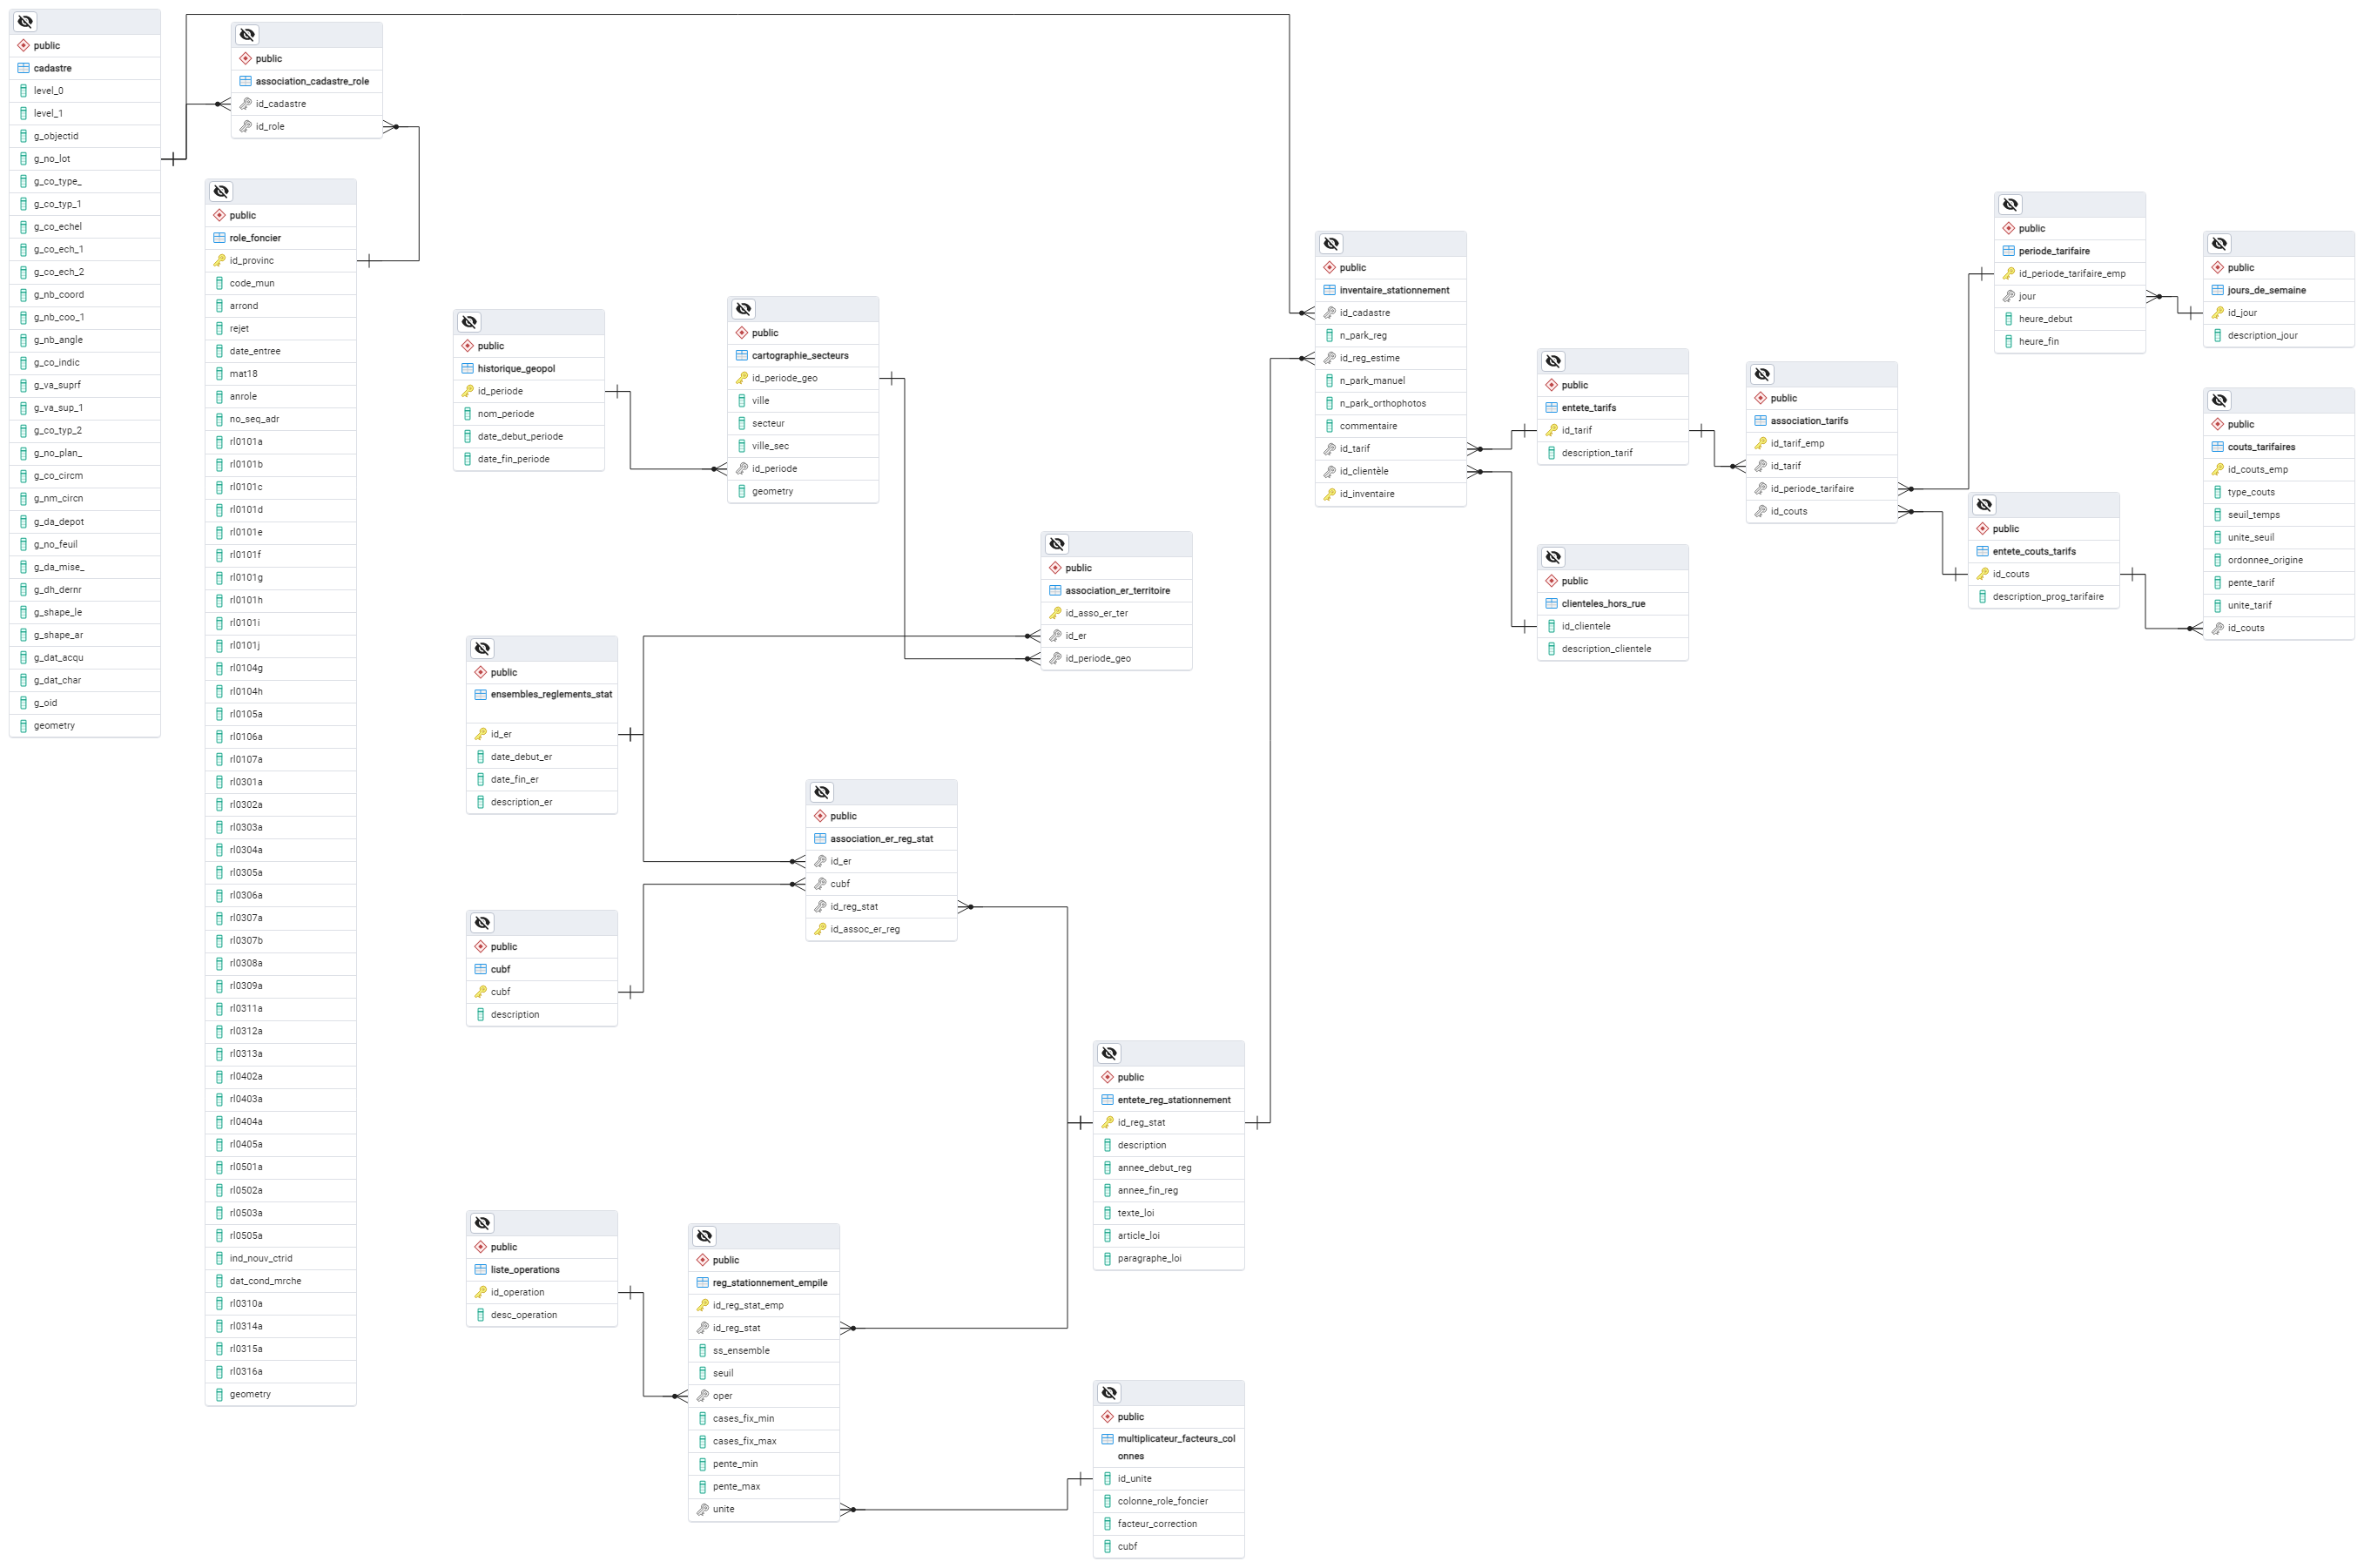
\includegraphics[trim={0cm 6cm 77.5cm 0cm},clip,height=20cm]{images/structure_base_de_donnee.png}
        \caption{Schéma relationnel pour le rôle foncier et le cadastre}
        \label{fig:offstreet_db_erd_input_data}
    \end{figure}
    \FloatBarrier
    
    \subsection{Calcul du nombre de places par méthode réglementaire}
        \subsubsection{Logigramme de la méthode globale}
        \subsubsection{Vérification de la base de données de stationnement}
            \paragraph{Validation des périodes de validité}
            \paragraph{Validation de couverture de l'ensemble des \ac{CUBF}}
        \subsubsection{Expansion des ensembles de règlements}
        \subsubsection{Sélection des propriétés à assigner: territoire et règlementation}
        \subsubsection{Gestion des propriétés non-assignées}
        \subsubsection{Inférence de la capacité de stationnement}
     
\section{Méthode d'inventaire hors rue basée sur les ortho-photographies}\label{sec:meth_orthophoto}
\section{Interface de programmation applicative}\label{sec:meth_API}
\section{Interface Web proposé} \label{sec:meth_interface_web}
\section{Méthode d'analyse} \label{sec:meth_analyse}
  \subsection{Analyse spatio temporelle de l'offre de stationnement}
  \subsection{Analyse spatio temporelle de la demande de stationnement}
  \subsection{Analyse d'utilisation de la ressource}
